\documentclass[11pt,a4paper]{article}

\usepackage[utf8]{inputenc}
\usepackage[T1]{fontenc}
\usepackage[indonesian]{babel}
\usepackage{lmodern}
\usepackage[a4paper,margin=2.5cm]{geometry}
\usepackage{graphicx}
\usepackage{float}
\usepackage{booktabs}
\usepackage{longtable}
\usepackage{array}
\usepackage{tabularx}
\usepackage{xcolor}
\usepackage{listings}
\usepackage{pdflscape}
\usepackage{caption}
\usepackage{titlesec}
\usepackage{cite}
\usepackage{tikz}
\usetikzlibrary{positioning,calc,backgrounds}
\usepackage[hidelinks]{hyperref}
\usepackage{xurl}

\captionsetup{font=small,labelfont=bf}

% garis horizontal di bawah setiap judul dan subjudul
\titleformat{\section}{\Large\bfseries}{\thesection}{1em}{}[{\vspace{2pt}\titlerule[0.8pt]}]
\titleformat{\subsection}{\large\bfseries}{\thesubsection}{1em}{}[{\vspace{1pt}\titlerule[0.4pt]}]
\setlength{\parskip}{0.5em}
\setlength{\parindent}{0pt}
\renewcommand{\arraystretch}{1.25}

% ---------------------------------------------------------------- listing SPARQL
\lstdefinelanguage{SPARQL}{
  morekeywords={PREFIX,SELECT,DISTINCT,WHERE,FILTER,OPTIONAL,UNION,MINUS,ORDER,BY,ASC,DESC},
  sensitive=true,
  morestring=[b]",
}
\lstset{
  language=SPARQL,
  basicstyle=\ttfamily\footnotesize,
  keywordstyle=\color{magenta!70!black}\bfseries,
  commentstyle=\color{gray},
  stringstyle=\color{green!40!black},
  frame=single,
  rulecolor=\color{gray!60},
  backgroundcolor=\color{gray!5},
  breaklines=true,
  columns=fullflexible,
  keepspaces=true,
  showstringspaces=false,
  xleftmargin=2pt,
  xrightmargin=2pt,
}

% ---------------------------------------------------------------- gaya diagram silsilah
\tikzset{
  p/.style={draw, rounded corners=2pt, align=center, text width=2.75cm,
            minimum height=1.05cm, font=\scriptsize, inner sep=2pt, line width=0.6pt,
            execute at begin node={\hyphenpenalty=10000\exhyphenpenalty=10000}},
  lk/.style={p, draw=black, fill=blue!6},
  pr/.style={p, draw=black, fill=red!6},
  sultan/.style={p, draw=black, fill=yellow!30, line width=1.4pt},
  nikah/.style={line width=1.2pt},
  turun/.style={line width=0.6pt},
  turunb/.style={line width=0.6pt, dashed, draw=black},
}
% \nikah{suami/istri kiri}{suami/istri kanan}{nama titik tengah}
\newcommand{\nikah}[3]{%
  \draw[nikah] (#1.east) -- (#2.west) coordinate[midway] (#3);}
% \turun[gaya]{titik asal}{tinggi bar (cm di bawah asal)}{daftar anak}
\newcommand{\turun}[4][turun]{%
  \foreach \c in {#4} {\draw[#1] (#2) -- ++(0,-#3) -| (\c.north);}}

\begin{document}

% ================================================================ JUDUL
\begin{titlepage}
  \centering
  \vspace*{2cm}
  {\Large\bfseries LAPORAN EVALUASI 2\\[0.3em] REPRESENTASI PENGETAHUAN DAN PENALARAN\par}
  \vspace{1.2cm}
  {\LARGE\bfseries Ontologi Silsilah Keluarga\\[0.2em] Kasultanan Ngayogyakarta Hadiningrat\\[0.2em] dengan Prot\'eg\'e dan SPARQL\par}
  \vspace{2cm}
  {\large Kelompok 13\par}
  \vspace{0.8cm}
  \begin{tabular}{ll}
    \toprule
    \textbf{Nama} & \textbf{NRP} \\
    \midrule
    Gilbran Mahdavikia Raja & 5025241134 \\
    Nabila Shafa Rahayu & 5025241150 \\
    Rahma Sakinah & 5025241222 \\
    \bottomrule
  \end{tabular}
  \vfill
  {\large Departemen Teknik Informatika\\ Institut Teknologi Sepuluh Nopember\\ 2026\par}
\end{titlepage}

\tableofcontents
\newpage

% ================================================================ PENDAHULUAN
\section*{Ringkasan Ontologi}
\addcontentsline{toc}{section}{Ringkasan Ontologi}

Ontologi ini memodelkan silsilah keluarga Kasultanan Ngayogyakarta Hadiningrat, mulai dari Sri Sultan
Hamengku Buwono I sampai cucu Sri Sultan Hamengku Bawono Ka 10. Sumber utama adalah situs resmi Keraton
Yogyakarta, \url{https://www.kratonjogja.id/} \cite{kj-hb1,kj-hb2,kj-hb3,kj-hb4,kj-hb5,kj-hb6,kj-hb7,kj-hb8,kj-hb9,kj-bertakhta,kj-hayu,kj-maduretno,kj-hemas,kj-pepatih,kj-nisaka}.
Data yang tidak dimuat di situs tersebut, misalnya tahun lahir, urutan istri, dan ayah dari Kanjeng Ratu Alit,
diambil dari sumber pendukung \cite{wiki-hb8,wiki-hb9,wiki-hb10,wiki-dipo,wiki-hemas,ra-y6,ra-y7,ra-y8}.
Data yang tidak ditemukan di sumber mana pun dibiarkan kosong.

\begin{itemize}
  \item \textbf{File ontologi:} \texttt{ontologi\_kasultanan\_yogyakarta.owl} (RDF/XML).
  \item \textbf{Namespace:} \url{http://www.semanticweb.org/mamahda/ontologies/2026/10/kasultanan-yogyakarta#}.
  \item \textbf{Isi:} 7 kelas, 14 \textit{object property}, 13 \textit{data property}, dan 69 individu:
        47 orang dari 12 generasi berurutan, 21 pernikahan, dan 1 kerajaan.
  \item \textbf{Pernikahan dengan data anak:} 15 pasangan (syarat minimal 4).
  \item \textbf{Perangkat:} Prot\'eg\'e 5.6.9, \textit{reasoner} HermiT 1.4.3, dan \textit{plugin} Snap SPARQL Query 6.0.0.
\end{itemize}

\begin{figure}[H]
  \centering
  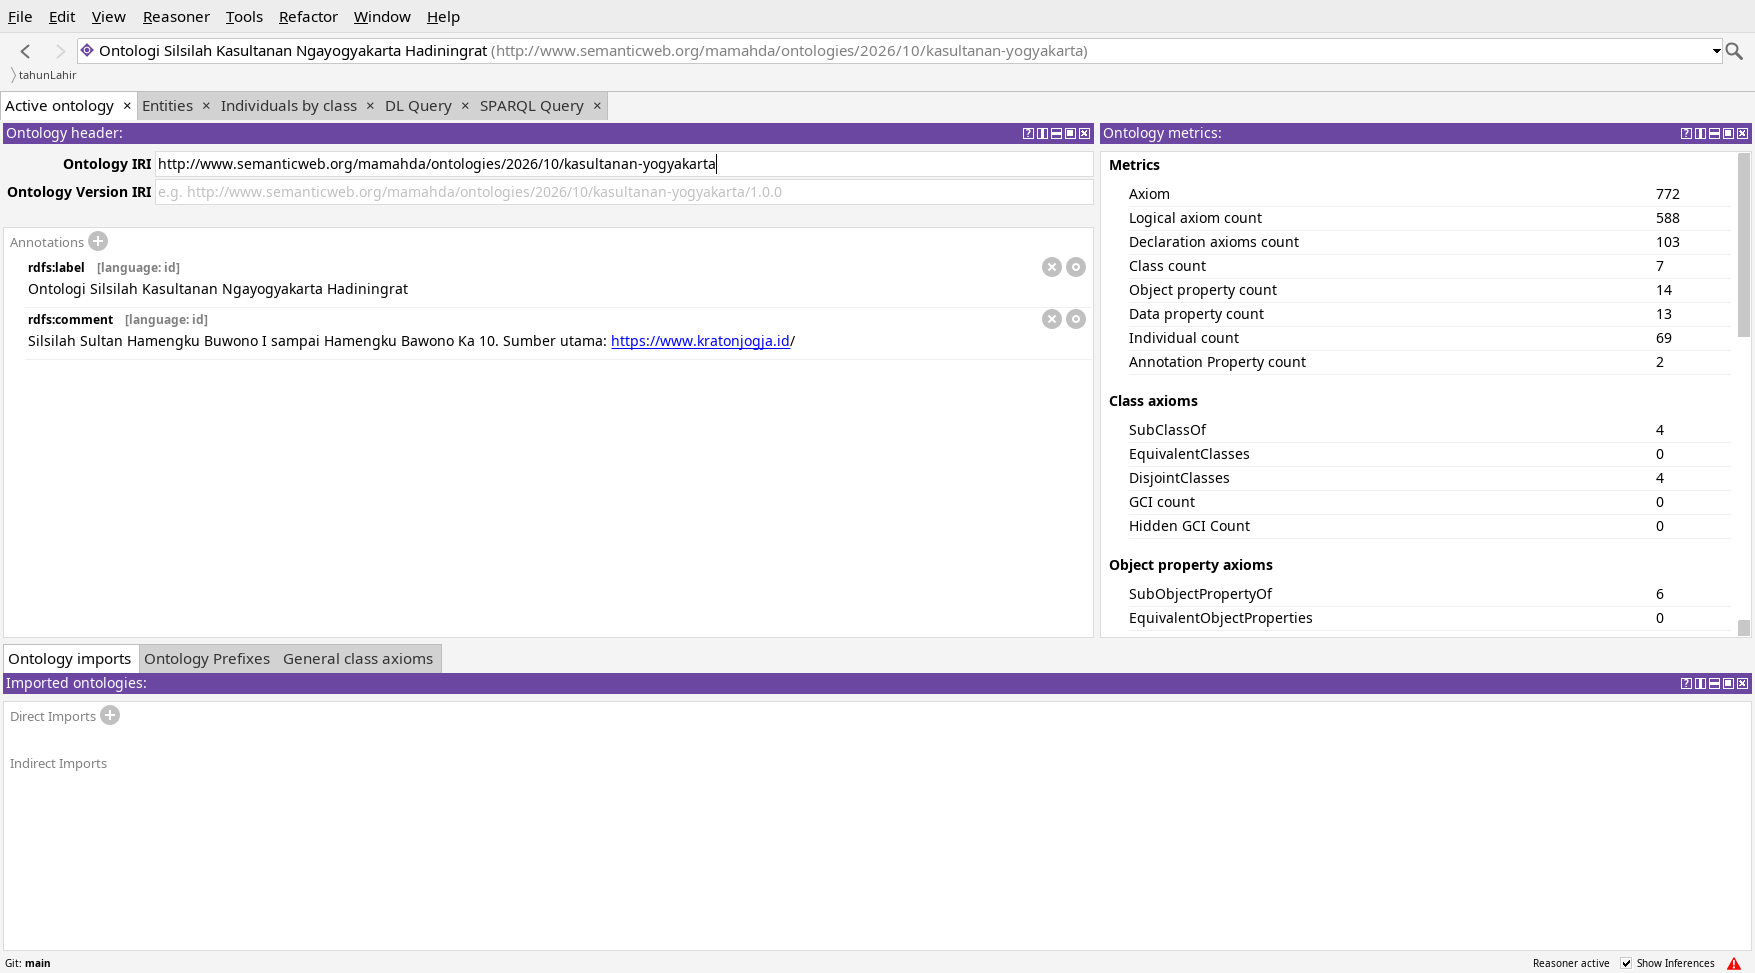
\includegraphics[width=\textwidth]{gambar/active_ontology.png}
  \caption{Tab \textit{Active ontology} di Prot\'eg\'e: IRI ontologi dan metrik (7 kelas, 14 \textit{object property}, 13 \textit{data property}, 69 individu).}
  \label{fig:metrik}
\end{figure}

% ================================================================ 1. DIAGRAM SILSILAH
\section{Diagram Silsilah}

Diagram silsilah dibagi menjadi dua bagian supaya tetap terbaca: Gambar~\ref{fig:silsilah1} memuat generasi
Sunan Amangkurat IV sampai Sri Sultan Hamengku Buwono VII, dan Gambar~\ref{fig:silsilah2} memuat Sri Sultan
Hamengku Buwono VII sampai cucu Sri Sultan Hamengku Bawono Ka 10. Setiap kotak mencantumkan nomor referensi
asal datanya.

\textbf{Keterangan diagram:} kotak \colorbox{yellow!30}{kuning bergaris tebal} = Sultan (kelas \texttt{Penguasa});
kotak \colorbox{blue!6}{biru} = laki-laki; kotak \colorbox{red!6}{merah muda} = perempuan; garis horizontal tebal = pernikahan;
garis tipis dari tengah garis pernikahan = keturunan. Garis putus-putus pada Gambar~\ref{fig:silsilah2}
menandai keturunan GPAA Mangkubumi yang menikah dengan sepupunya, Sri Sultan Hamengku Buwono VIII.

% ---------------------------------------------------------------- Gambar 1
\begin{landscape}
\begin{figure}[p]
\centering
\resizebox{\linewidth}{!}{%
\begin{tikzpicture}[x=1cm,y=1cm]
  % generasi 0
  \node[lk] (AM4) at (8,0)  {Sunan Amangkurat IV \cite{kj-hb1}};
  \node[pr] (TEJ) at (12,0) {Mas Ayu Tejawati\\(garwa selir) \cite{kj-hb1}};
  % generasi 1
  \node[sultan] (HB1) at (10,-2.2) {\textbf{HB I}\\BRM Sujono\\1717--1792 \cite{kj-hb1}};
  \node[pr] (KAD) at (14,-2.2) {GKR Kadipaten\\(permaisuri ke-2) \cite{kj-hb2}};
  % generasi 2
  \node[sultan] (HB2) at (12,-4.4) {\textbf{HB II}\\RM Sundoro\\1750--1828 \cite{kj-hb2}};
  \node[pr] (KED) at (16,-4.4) {GKR Kedhaton \cite{kj-hb3,kj-pepatih}};
  % generasi 3
  \node[lk] (DAN)  at (3,-6.6)  {KRA Danurejo II\\(Pepatih Dalem) \cite{kj-pepatih}};
  \node[pr] (HANG) at (7,-6.6)  {GKR Hangger \cite{kj-pepatih}};
  \node[pr] (MANG) at (11,-6.6) {R.A. Mangkarawati\\(garwa selir) \cite{kj-hb3,wiki-dipo}};
  \node[sultan] (HB3) at (15,-6.6) {\textbf{HB III}\\RM Surojo\\1769--1814 \cite{kj-hb3}};
  \node[pr] (HAG)  at (19,-6.6) {GKR Hageng \cite{kj-hb4}};
  % generasi 4
  \node[lk] (DIPO) at (12,-8.8) {P. Diponegoro\\RM Antawirya\\1785--1855 \cite{kj-hb3,wiki-dipo}};
  \node[sultan] (HB4) at (17,-8.8) {\textbf{HB IV}\\GRM Ibnu Jarot\\1804--1823 \cite{kj-hb4}};
  \node[pr] (KEN4) at (21,-8.8) {GKR Kencono \cite{kj-hb4,kj-hb5}};
  % generasi 5
  \node[pr] (KEN5) at (3,-11)  {GKR Kencono\\(permaisuri ke-1,\\tidak berputra) \cite{kj-hb5}};
  \node[sultan] (HB5) at (7,-11)  {\textbf{HB V}\\GRM Gatot Menol\\1821--1855 \cite{kj-hb5}};
  \node[pr] (SEK)  at (11,-11) {GKR Sekar Kedhaton\\(permaisuri ke-2) \cite{kj-hb5}};
  \node[pr] (HBW)  at (15,-11) {GKR Hamengku Buwono\\(permaisuri ke-1,\\putri PB VIII) \cite{kj-hb6}};
  \node[sultan] (HB6) at (19,-11) {\textbf{HB VI}\\GRM Mustojo\\1821--1877 \cite{kj-hb6}};
  \node[pr] (SUL)  at (23,-11) {GKR Sultan\\(permaisuri ke-2) \cite{kj-hb7}};
  % generasi 6
  \node[lk] (SURY) at (9,-13.2)  {KPH Suryaning Ngalaga\\GRM Timur Muhammad \cite{kj-hb6}};
  \node[sultan] (HB7) at (19,-13.2) {\textbf{HB VII}\\GRM Murtejo\\1839--1921 \cite{kj-hb7}};
  \node[lk] (GPAA) at (23,-13.2) {GPAA Mangkubumi \cite{ra-y6,wiki-hb8}};

  \begin{scope}[on background layer]
    \nikah{AM4}{TEJ}{m0}   \turun{m0}{1.1}{HB1}
    \nikah{HB1}{KAD}{m1}   \turun{m1}{1.1}{HB2}
    \nikah{HB2}{KED}{m2}   \turun{m2}{1.1}{HANG,HB3}
    \nikah{DAN}{HANG}{m3a}
    \nikah{MANG}{HB3}{m3b} \turun{m3b}{1.1}{DIPO}
    \nikah{HB3}{HAG}{m3c}  \turun{m3c}{1.1}{HB4}
    \nikah{HB4}{KEN4}{m4}  \turun{m4}{1.1}{HB5,HB6}
    \nikah{KEN5}{HB5}{m5a}
    \nikah{HB5}{SEK}{m5b}  \turun{m5b}{1.1}{SURY}
    \nikah{HBW}{HB6}{m6a}
    \nikah{HB6}{SUL}{m6b}  \turun{m6b}{1.1}{HB7,GPAA}
  \end{scope}
\end{tikzpicture}}
\caption{Silsilah bagian 1: Sunan Amangkurat IV sampai Sri Sultan Hamengku Buwono VII (generasi 0--6).}
\label{fig:silsilah1}
\end{figure}
\end{landscape}

% ---------------------------------------------------------------- Gambar 2
\begin{landscape}
\begin{figure}[p]
\centering
\resizebox{\linewidth}{!}{%
\begin{tikzpicture}[x=1cm,y=1cm]
  % generasi 6
  \node[pr] (HEM7) at (2,0)  {GKR Hemas\\(permaisuri HB VII) \cite{kj-hb8}};
  \node[sultan] (HB7) at (6,0)  {\textbf{HB VII}\\GRM Murtejo\\1839--1921 \cite{kj-hb7}};
  \node[lk] (GPAA) at (17,0) {GPAA Mangkubumi\\(putra HB VI,\\adik HB VII) \cite{ra-y6,wiki-hb8}};
  % generasi 7
  \node[pr] (KAT) at (4,-2.4)  {RA Siti Katina\\(istri ke-1, m. 1907) \cite{wiki-hb8,ra-y8}};
  \node[sultan] (HB8) at (8,-2.4)  {\textbf{HB VIII}\\GRM Sujadi\\1880--1939 \cite{kj-hb8}};
  \node[pr] (KUS) at (12,-2.4) {Kanjeng Ratu Alit\\RAj Kustilah\\(istri ke-5) \cite{kj-hb9,wiki-hb8}};
  % generasi 8
  \node[pr] (PIN) at (9,-4.8)  {KRAy Pintakapurnama\\(istri ke-1, m. 1940) \cite{wiki-hb9}};
  \node[sultan] (HB9) at (13,-4.8) {\textbf{HB IX}\\GRM Dorojatun\\1912--1988 \cite{kj-hb9}};
  \node[pr] (WIN) at (17,-4.8) {KRAy Windyaningrum\\(istri ke-2, m. 1943) \cite{kj-bertakhta,wiki-hb9}};
  % generasi 9
  \node[sultan] (HB10) at (15,-7.2) {\textbf{HB Ka 10}\\BRM Herjuno Darpito\\l. 1946 \cite{kj-bertakhta}};
  \node[pr] (HEM)  at (19,-7.2) {GKR Hemas\\l. 1952 \cite{kj-hemas,wiki-hemas}};
  % generasi 10
  \node[lk] (WIR) at (2,-9.6)    {KPH Wironegoro \cite{wiki-hb10}};
  \node[pr] (MB)  at (5.2,-9.6)  {GKR Mangkubumi\\l. 1972 \cite{kj-bertakhta,wiki-hb10}};
  \node[pr] (CK)  at (8.4,-9.6)  {GKR Condrokirono\\l. 1975 \cite{kj-bertakhta,wiki-hb10}};
  \node[pr] (MD)  at (14.8,-9.6) {GKR Maduretno\\l. 1978 \cite{kj-maduretno,wiki-hb10}};
  \node[lk] (PUR) at (18,-9.6)   {KPH Purbodiningrat \cite{kj-maduretno}};
  \node[pr] (HY)  at (21.2,-9.6) {GKR Hayu\\l. 1982 \cite{kj-hayu,wiki-hb10}};
  \node[lk] (NOT) at (24.4,-9.6) {KPH Notonegoro\\(m. 2013) \cite{kj-hayu}};
  \node[pr] (BD)  at (27.6,-9.6) {GKR Bendara\\l. 1986 \cite{kj-bertakhta,wiki-hb10}};
  \node[lk] (YUD) at (30.8,-9.6) {KPH Yudanegara \cite{kj-nisaka}};
  % generasi 11
  \node[pr] (ART) at (1.4,-12)  {RAj Artie Ayya\\Fatimasari \cite{wiki-hb10}};
  \node[lk] (DRA) at (4.6,-12)  {RM Drasthya\\Wironegoro \cite{wiki-hb10}};
  \node[lk] (MAR) at (8.4,-12)  {RM Gusthilantika\\Marrel Suryokusumo \cite{wiki-hb10}};
  \node[lk] (MAN) at (22.8,-12) {RM Manteyyo Kuncoro\\Suryonegoro, l. 2019 \cite{kj-hayu}};
  \node[pr] (NIS) at (27.6,-12) {RAj Nisaka Irdina\\Yudanegara \cite{kj-nisaka}};
  \node[lk] (RAD) at (30.8,-12) {RM Radityo Mandhala\\Yudanegara \cite{wiki-hb10}};

  \begin{scope}[on background layer]
    \nikah{HEM7}{HB7}{n7}   \turun{n7}{1.0}{HB8}
    \turun[turunb]{GPAA.south}{1.05}{KAT,KUS}
    \nikah{KAT}{HB8}{n8a}
    \nikah{HB8}{KUS}{n8b}   \turun{n8b}{1.2}{HB9}
    \nikah{PIN}{HB9}{n9a}
    \nikah{HB9}{WIN}{n9b}   \turun{n9b}{1.2}{HB10}
    \nikah{HB10}{HEM}{n10}  \turun{n10}{1.2}{MB,CK,MD,HY,BD}
    \nikah{WIR}{MB}{n11a}   \turun{n11a}{1.2}{ART,DRA}
    \turun{CK.south}{0.7}{MAR}
    \nikah{MD}{PUR}{n11c}
    \nikah{HY}{NOT}{n11d}   \turun{n11d}{1.2}{MAN}
    \nikah{BD}{YUD}{n11e}   \turun{n11e}{1.2}{NIS,RAD}
  \end{scope}
\end{tikzpicture}}
\caption{Silsilah bagian 2: Sri Sultan Hamengku Buwono VII sampai cucu Sri Sultan Hamengku Bawono Ka 10 (generasi 6--11).
Garis putus-putus: putri-putri GPAA Mangkubumi, sepupu Sri Sultan Hamengku Buwono VIII.}
\label{fig:silsilah2}
\end{figure}
\end{landscape}

\subsection{Keterangan Sumber Silsilah}

\begin{longtable}{>{\raggedright\arraybackslash}p{3.2cm} >{\raggedright\arraybackslash}p{9.6cm} p{1.8cm}}
\caption{Keterangan data silsilah dan sumbernya.}\label{tab:sumber}\\
\toprule
\textbf{Bagian} & \textbf{Keterangan} & \textbf{Sumber} \\
\midrule
\endfirsthead
\toprule
\textbf{Bagian} & \textbf{Keterangan} & \textbf{Sumber} \\
\midrule
\endhead
HB I & Nama lahir BRM Sujono, lahir 5 Agustus 1717, putra Sunan Amangkurat IV dan garwa selir Mas Ayu Tejawati.
Dinobatkan 13 Maret 1755 dan wafat 24 Maret 1792. & \cite{kj-hb1} \\
HB II & RM Sundoro, lahir 7 Maret 1750, putra HB I dari permaisuri kedua GKR Kadipaten. Bertakhta 1792--1810,
1811--1812, dan 1826--1828, lalu wafat 3 Januari 1828. & \cite{kj-hb2} \\
HB III & RM Surojo, lahir 20 Februari 1769, putra HB II dan GKR Kedhaton. Wafat 3 November 1814. & \cite{kj-hb3} \\
GKR Hangger & Putri HB II dari garwa padmi GKR Kedhaton, menikah dengan Danurejo II. & \cite{kj-pepatih} \\
P. Diponegoro & Putra sulung HB III dari garwa selir. Nama ibu (R.A. Mangkarawati) serta tahun lahir dan wafat dari \cite{wiki-dipo}. & \cite{kj-hb3,wiki-dipo} \\
HB IV & GRM Ibnu Jarot, lahir 3 April 1804, putra HB III dan GKR Hageng, wafat 6 Desember 1823. Permaisurinya GKR Kencono. & \cite{kj-hb4} \\
HB V & GRM Gatot Menol, lahir 20 Januari 1821, putra HB IV dan GKR Kencono. Permaisuri pertama GKR Kencono (tidak berputra),
permaisuri kedua GKR Sekar Kedhaton. Wafat 5 Juni 1855. & \cite{kj-hb5} \\
KPH Suryaning Ngalaga & GRM Timur Muhammad, lahir dari permaisuri HB V setelah HB V wafat. & \cite{kj-hb5,kj-hb6} \\
HB VI & GRM Mustojo, lahir 10 Agustus 1821, adik HB V. Pada usia 27 tahun (sekitar 1848) menikah dengan GKR Kencono,
putri Paku Buwono VIII, yang bergelar GKR Hamengku Buwono. Wafat 20 Juli 1877. & \cite{kj-hb6} \\
HB VII & GRM Murtejo, lahir 4 Februari 1839, putra HB VI dari GKR Sultan (permaisuri kedua). Wafat 30 Desember 1921. & \cite{kj-hb7} \\
GPAA Mangkubumi & Putra HB VI dari Ratu Sultan, sehingga saudara seayah-seibu HB VII. & \cite{ra-y6,wiki-hb8} \\
HB VIII & GRM Sujadi, lahir 3 Maret 1880, putra HB VII dan GKR Hemas. Wafat 22 Oktober 1939. & \cite{kj-hb8} \\
Istri HB VIII & RA Siti Katina (istri ke-1, menikah 1907) dan RAj Kustilah/Kanjeng Ratu Alit (istri ke-5).
Keduanya putri GPAA Mangkubumi. & \cite{kj-hb9,wiki-hb8,ra-y8} \\
HB IX & GRM Dorojatun, lahir 12 April 1912, anak kesembilan HB VIII dari istri kelima, Kanjeng Ratu Alit. Wafat 2 Oktober 1988. & \cite{kj-hb9} \\
Istri HB IX & KRAy Pintakapurnama (menikah 1940) dan KRAy Windyaningrum (menikah 1943). & \cite{wiki-hb9} \\
HB Ka 10 & BRM Herjuno Darpito, lahir 2 April 1946, putra HB IX dan KRAy Windyaningrum. Bertakhta sejak 7 Maret 1989.
Permaisurinya GKR Hemas, dengan lima putri. & \cite{kj-bertakhta} \\
GKR Hemas & Nama lahir Tatiek Dradjad Suprihastuti, lahir 31 Oktober 1952. & \cite{kj-hemas,wiki-hemas} \\
Putri HB Ka 10 & Nama lahir dari \cite{kj-bertakhta}. Tahun lahir, suami, dan cucu dari \cite{wiki-hb10}. GKR Hayu
menikah dengan KPH Notonegoro pada 2013 dan berputra RM Manteyyo (lahir Agustus 2019) \cite{kj-hayu}. GKR Maduretno
menikah dengan KPH Purbodiningrat \cite{kj-maduretno}. & \cite{kj-bertakhta,wiki-hb10,kj-hayu,kj-maduretno} \\
RAj Nisaka Irdina & Putri GKR Bendara dan KPH Yudanegara. & \cite{kj-nisaka} \\
\bottomrule
\end{longtable}

\subsection{Perbedaan Data Antarsumber}

Beberapa sumber memberikan data yang berbeda. Tabel~\ref{tab:beda} mencatat perbedaan tersebut beserta versi yang
dipakai di ontologi. Data yang tidak ditemukan di sumber mana pun tidak diisi, misalnya tahun lahir para permaisuri
sebelum GKR Hemas, tahun lahir menantu HB Ka 10, dan ayah RM Gusthilantika Marrel Suryokusumo.

\begin{table}[H]
\centering
\caption{Perbedaan data antarsumber dan keputusan yang diambil.}
\label{tab:beda}
\small
\begin{tabularx}{\textwidth}{>{\raggedright\arraybackslash}p{2.3cm} >{\raggedright\arraybackslash}X >{\raggedright\arraybackslash}X >{\raggedright\arraybackslash}X}
\toprule
\textbf{Data} & \textbf{Versi A} & \textbf{Versi B} & \textbf{Keputusan} \\
\midrule
Ibu HB IV & ``GKR Hageng'' (halaman HB IV \cite{kj-hb4}); ``Ratu Ageng'' di \cite{kj-hb5} & ``GKR Kencono'' (halaman HB III \cite{kj-hb3}) &
Dipakai GKR Hageng; nama GKR Kencono dicatat di \texttt{gelar}. \\
Urutan GKR Sultan sebagai istri HB VI & Permaisuri kedua \cite{kj-hb7} & Istri pertama \cite{ra-y6} &
Dipakai versi \cite{kj-hb7} (\texttt{urutanPernikahan} = 2). Secara kronologis versi \cite{ra-y6} lebih cocok karena HB VII lahir 1839,
sebelum HB VI menikahi GKR Hamengku Buwono ($\pm$1848). \\
Ibu HB VIII & GKR Hemas \cite{kj-hb8,wiki-hb8} & ``Ratu Mas'', istri ke-9 HB VII \cite{ra-y7} & Dipakai GKR Hemas. \\
Nama kecil Diponegoro & RM Antawirya \cite{kj-hb3} & BRM Mustahar \cite{wiki-dipo} & Dipakai RM Antawirya; BRM Mustahar dicatat di \texttt{gelar}. \\
\bottomrule
\end{tabularx}
\end{table}

% ================================================================ 2. PEMBAGIAN TUGAS
\section{Pembagian Tugas}

\begin{table}[H]
\centering
\caption{Pembagian tugas anggota kelompok.}
\label{tab:tugas}
\begin{tabularx}{\textwidth}{l l >{\raggedright\arraybackslash}X}
\toprule
\textbf{Nama} & \textbf{NRP} & \textbf{Tugas} \\
\midrule
Gilbran Mahdavikia Raja & 5025241134 & Pengumpulan dan verifikasi data HB I--HB V, tabel perbedaan sumber \\
Nabila Shafa Rahayu & 5025241150 & Pengumpulan dan verifikasi data HB VI--HB IX, pembangunan ontologi di Prot\'eg\'e, penyusunan dan pengujian query SPARQL \\
Rahma Sakinah & 5025241222 & Pengumpulan dan verifikasi data keluarga HB Ka 10, diagram silsilah, penyusunan laporan dan daftar pustaka \\
\bottomrule
\end{tabularx}
\end{table}

% ================================================================ 3. HIERARKI KELAS
\section{Hierarki Kelas}

Ontologi memiliki tujuh kelas. \texttt{LakiLaki} dan \texttt{Perempuan} dinyatakan saling \textit{disjoint}, begitu juga
\texttt{Orang}, \texttt{Pernikahan}, dan \texttt{Kerajaan}. Pernikahan dimodelkan sebagai kelas tersendiri (reifikasi)
agar urutan pernikahan dan tahun menikah dapat disimpan, karena keduanya merupakan atribut pernikahan, bukan atribut orang.

\begin{figure}[H]
\centering
\begin{tikzpicture}[
    k/.style={draw, rounded corners=2pt, fill=yellow!20, font=\small\ttfamily, inner sep=4pt},
    level distance=1.4cm, sibling distance=3.2cm, edge from parent/.style={draw, -latex}]
  \node[k] {owl:Thing}
    child {node[k] {Kerajaan}}
    child {node[k] {Orang}
      child {node[k] {LakiLaki} child {node[k] {Penguasa}}}
      child {node[k] {Perempuan} child {node[k] {Permaisuri}}}}
    child {node[k] {Pernikahan}};
\end{tikzpicture}
\caption{Hierarki kelas ontologi.}
\label{fig:hierarki}
\end{figure}

\begin{table}[H]
\centering
\caption{Deskripsi kelas.}
\label{tab:kelas}
\begin{tabularx}{\textwidth}{l l >{\raggedright\arraybackslash}X}
\toprule
\textbf{Kelas} & \textbf{Superkelas} & \textbf{Keterangan} \\
\midrule
\texttt{Orang} & \texttt{owl:Thing} & Manusia anggota silsilah \\
\texttt{LakiLaki} & \texttt{Orang} & Orang berjenis kelamin laki-laki; \textit{disjoint} dengan \texttt{Perempuan} \\
\texttt{Perempuan} & \texttt{Orang} & Orang berjenis kelamin perempuan \\
\texttt{Penguasa} & \texttt{LakiLaki} & Sultan yang pernah bertakhta di Kasultanan Yogyakarta (HB I--HB Ka 10) \\
\texttt{Permaisuri} & \texttt{Perempuan} & Garwa padmi (permaisuri) Sultan \\
\texttt{Pernikahan} & \texttt{owl:Thing} & Reifikasi pernikahan: menyimpan suami, istri, urutan, dan tahun menikah \\
\texttt{Kerajaan} & \texttt{owl:Thing} & Kerajaan; berisi satu individu, \texttt{KasultananYogyakarta} \\
\bottomrule
\end{tabularx}
\end{table}

\begin{figure}[H]
\centering
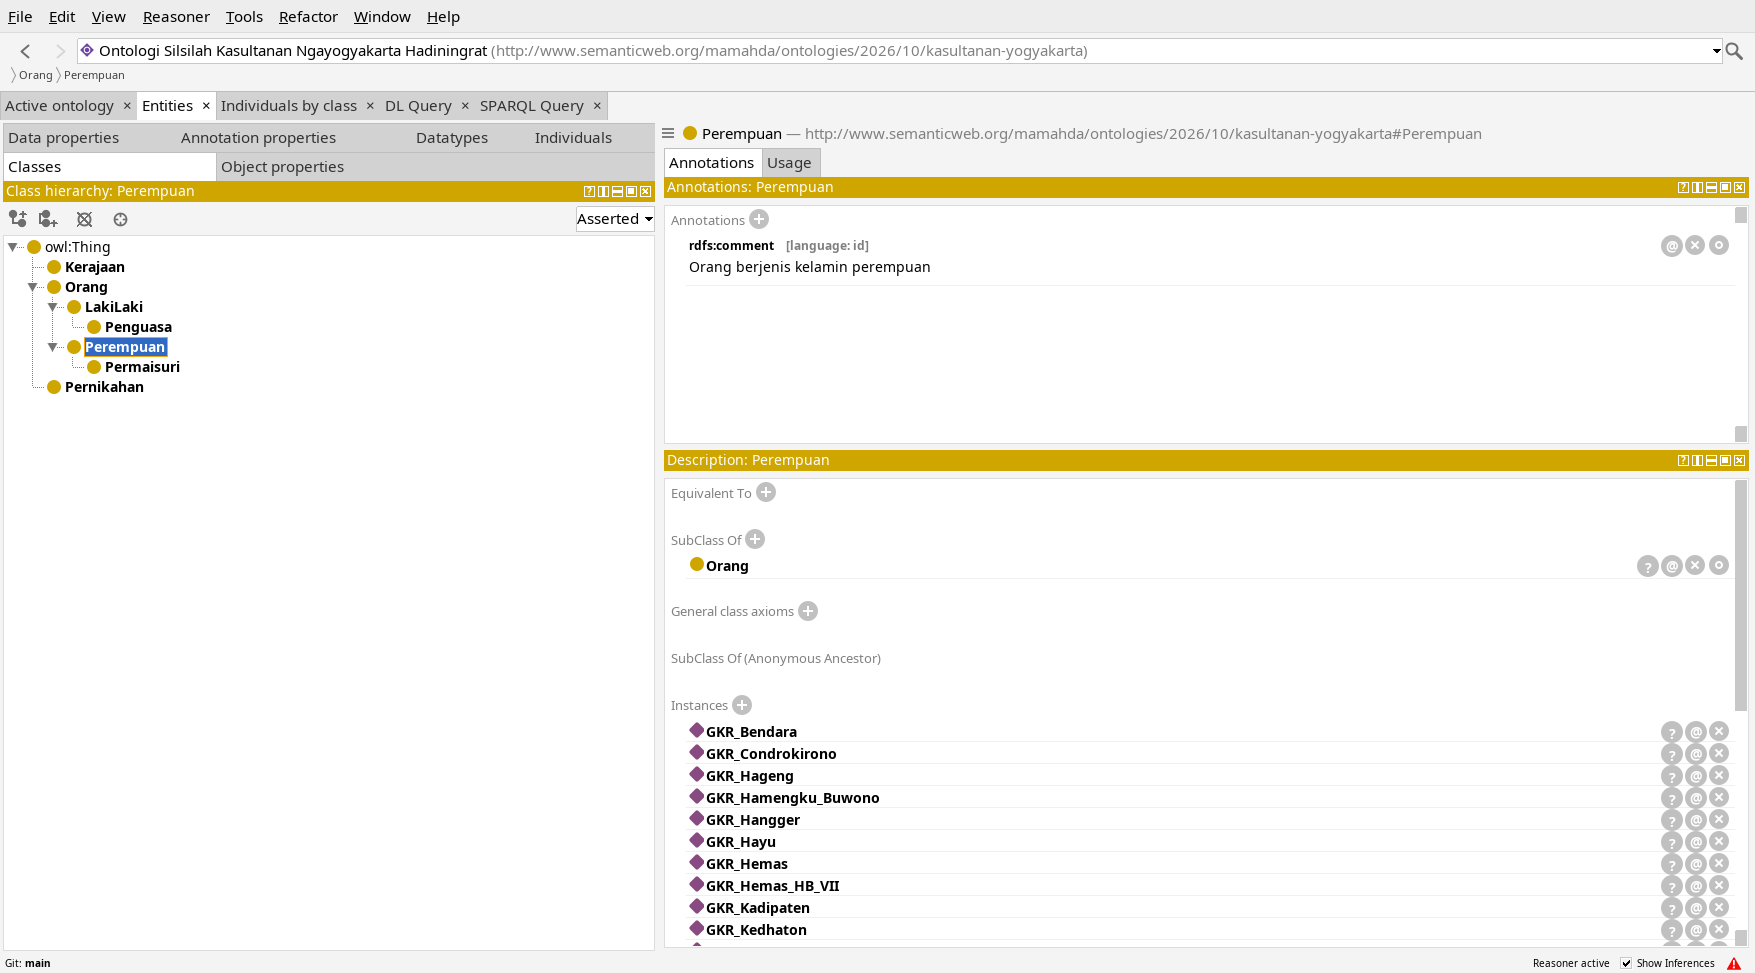
\includegraphics[width=\textwidth]{gambar/kelas_hierarki.png}
\caption{Hierarki kelas di Prot\'eg\'e. Kelas \texttt{Perempuan} dipilih sehingga terlihat superkelas dan individunya.}
\label{fig:ss-kelas}
\end{figure}

% ================================================================ 4. TABEL PROPERTY
\section{Tabel Property}

\subsection{Object Property}

\begin{table}[H]
\centering
\caption{Daftar \textit{object property}.}
\label{tab:objprop}
\small
\begin{tabularx}{\textwidth}{l l l l >{\raggedright\arraybackslash}X}
\toprule
\textbf{Property} & \textbf{Domain} & \textbf{Range} & \textbf{Karakteristik} & \textbf{Inverse / Super-property} \\
\midrule
\texttt{punyaAyah} & Orang & LakiLaki & \textbf{Functional} & inverse \texttt{ayahDari}; sub \texttt{punyaOrangTua} \\
\texttt{punyaIbu} & Orang & Perempuan & \textbf{Functional} & inverse \texttt{ibuDari}; sub \texttt{punyaOrangTua} \\
\texttt{ayahDari} & LakiLaki & Orang & \textbf{Inverse functional} & sub \texttt{punyaAnak} \\
\texttt{ibuDari} & Perempuan & Orang & \textbf{Inverse functional} & sub \texttt{punyaAnak} \\
\texttt{punyaOrangTua} & Orang & Orang & -- & inverse \texttt{punyaAnak}; sub \texttt{punyaLeluhur} \\
\texttt{punyaAnak} & Orang & Orang & -- & sub \texttt{punyaKeturunan} \\
\texttt{punyaLeluhur} & Orang & Orang & \textbf{Transitive} & inverse \texttt{punyaKeturunan} \\
\texttt{punyaKeturunan} & Orang & Orang & \textbf{Transitive} & -- \\
\texttt{menikahDengan} & Orang & Orang & Symmetric & -- \\
\texttt{suami} & Pernikahan & LakiLaki & Functional & -- \\
\texttt{istri} & Pernikahan & Perempuan & Functional & -- \\
\texttt{digantikanOleh} & Penguasa & Penguasa & \textbf{Functional} & inverse \texttt{menggantikan} \\
\texttt{menggantikan} & Penguasa & Penguasa & \textbf{Inverse functional} & -- \\
\texttt{memerintah} & Penguasa & Kerajaan & -- & -- \\
\bottomrule
\end{tabularx}
\end{table}

Kondisi yang memenuhi ketentuan \textit{functional}, \textit{inverse functional}, dan \textit{transitive}:
\begin{itemize}
  \item \textbf{Functional:} setiap orang hanya memiliki satu ayah (\texttt{punyaAyah}) dan satu ibu (\texttt{punyaIbu}).
        Setiap Sultan hanya memiliki satu penerus takhta langsung (\texttt{digantikanOleh}).
  \item \textbf{Inverse functional:} \texttt{ayahDari} dan \texttt{ibuDari}. Jika $X$ \texttt{ayahDari} $Z$ dan $Y$ \texttt{ayahDari} $Z$,
        maka $X = Y$, karena seorang anak hanya memiliki satu ayah. Begitu pula \texttt{menggantikan}: seorang Sultan hanya
        digantikan oleh satu Sultan.
  \item \textbf{Transitive:} \texttt{punyaLeluhur}. HB Ka 10 \texttt{punyaOrangTua} HB IX dan HB IX \texttt{punyaOrangTua} HB VIII,
        sehingga \textit{reasoner} menyimpulkan HB Ka 10 \texttt{punyaLeluhur} HB VIII, dan seterusnya sampai HB I.
\end{itemize}

\begin{figure}[H]
\centering
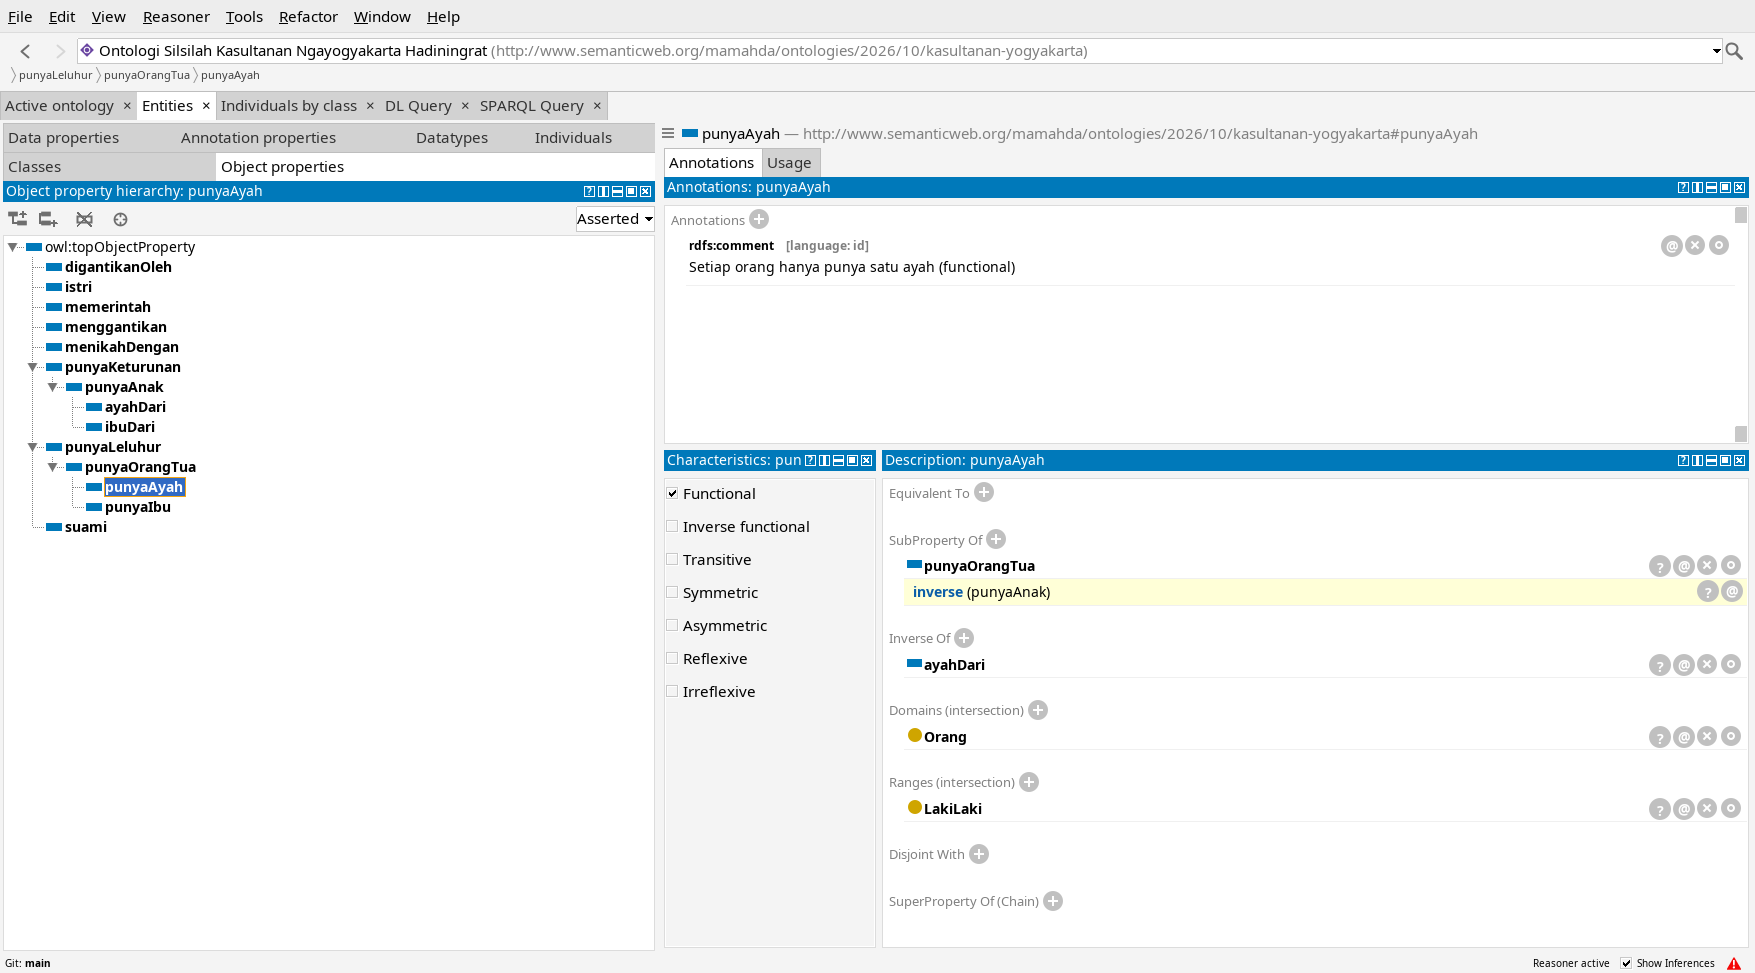
\includegraphics[width=\textwidth]{gambar/op_punyaAyah.png}
\caption{\texttt{punyaAyah} dengan karakteristik \textit{Functional}, \textit{sub-property} dari \texttt{punyaOrangTua}, dan \textit{inverse} dari \texttt{ayahDari}.}
\label{fig:ss-punyaAyah}
\end{figure}

\begin{figure}[H]
\centering
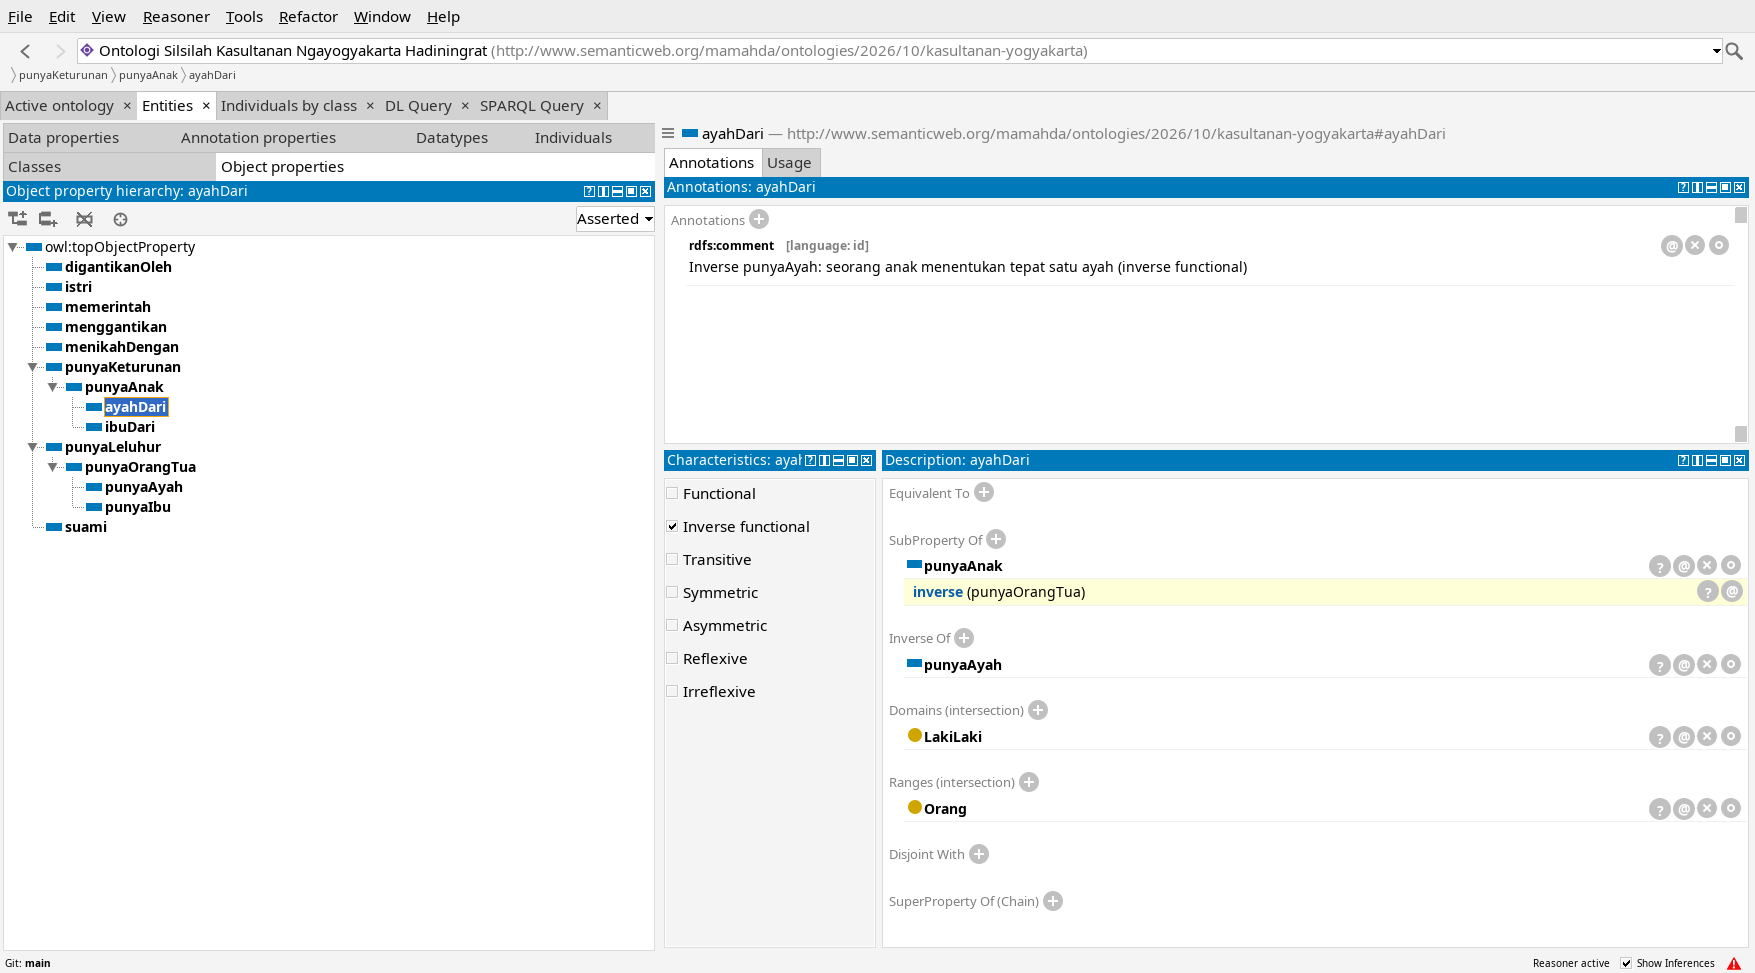
\includegraphics[width=\textwidth]{gambar/op_ayahDari.png}
\caption{\texttt{ayahDari} dengan karakteristik \textit{Inverse functional}.}
\label{fig:ss-ayahDari}
\end{figure}

\begin{figure}[H]
\centering
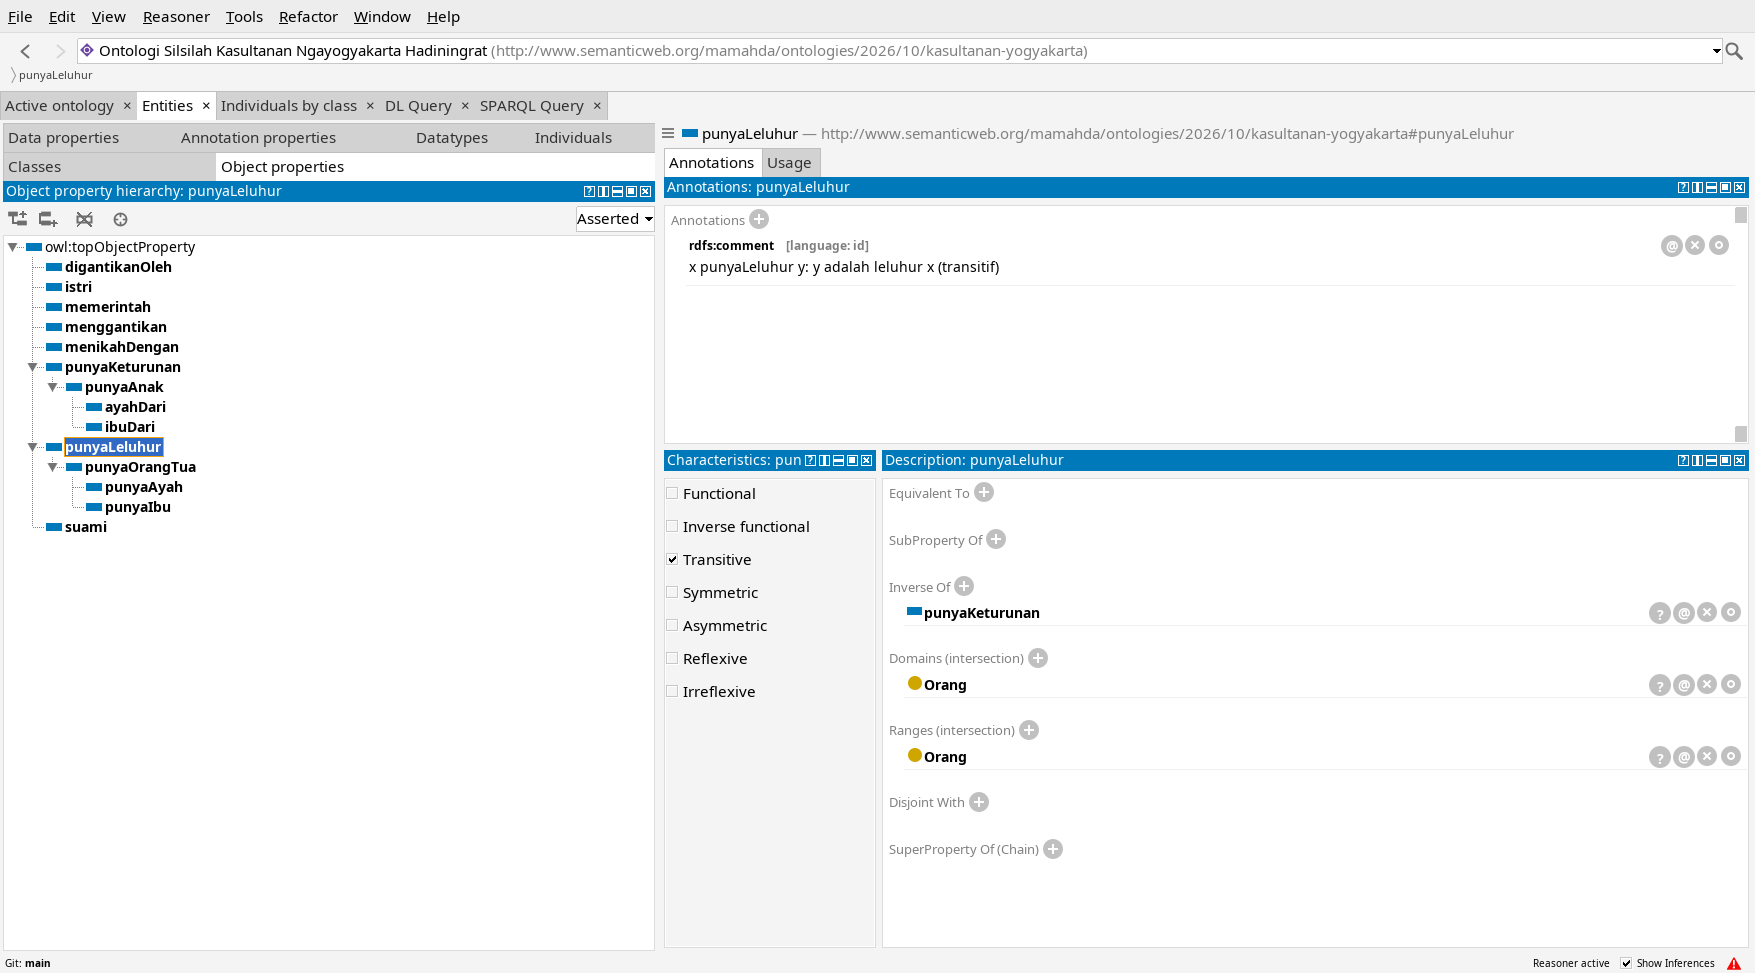
\includegraphics[width=\textwidth]{gambar/op_punyaLeluhur.png}
\caption{\texttt{punyaLeluhur} dengan karakteristik \textit{Transitive}.}
\label{fig:ss-punyaLeluhur}
\end{figure}

\subsection{Data Property}

\begin{table}[H]
\centering
\caption{Daftar \textit{data property}.}
\label{tab:dataprop}
\small
\begin{tabularx}{\textwidth}{l l l c >{\raggedright\arraybackslash}X}
\toprule
\textbf{Property} & \textbf{Domain} & \textbf{Range} & \textbf{Functional} & \textbf{Keterangan} \\
\midrule
\texttt{nama} & Orang & xsd:string & ya & Nama/gelar utama \\
\texttt{namaKecil} & Orang & xsd:string & -- & Nama lahir \\
\texttt{gelar} & Orang & xsd:string & -- & Gelar atau nama lain \\
\texttt{jenisKelamin} & Orang & xsd:string & ya & ``Laki-laki'' atau ``Perempuan'' \\
\texttt{tahunLahir} & Orang & xsd:integer & ya & Tahun lahir (Masehi) \\
\texttt{tahunWafat} & Orang & xsd:integer & ya & Tahun wafat (Masehi) \\
\texttt{tahunMulaiBerkuasa} & Penguasa & xsd:integer & ya & Tahun pertama kali naik takhta \\
\texttt{tahunAkhirBerkuasa} & Penguasa & xsd:integer & -- & Tahun akhir pemerintahan \\
\texttt{urutanPenguasa} & Penguasa & xsd:integer & ya & Urutan Sultan; 1 = HB I (generasi pertama) \\
\texttt{urutanPernikahan} & Pernikahan & xsd:integer & ya & Urutan istri bagi sang suami \\
\texttt{tahunMenikah} & Pernikahan & xsd:integer & ya & Tahun pernikahan \\
\texttt{namaKerajaan} & Kerajaan & xsd:string & ya & Nama kerajaan \\
\texttt{sumber} & -- & xsd:string & -- & Nomor referensi IEEE \\
\bottomrule
\end{tabularx}
\end{table}

Semua tahun disimpan sebagai \texttt{xsd:integer}, bukan \texttt{xsd:gYear} atau \texttt{xsd:date}, karena kedua tipe
tersebut tidak termasuk \textit{OWL 2 datatype map} sehingga tidak dapat diproses oleh HermiT. Tipe \texttt{xsd:integer}
juga memudahkan perbandingan dan pengurutan di SPARQL.

\begin{figure}[H]
\centering
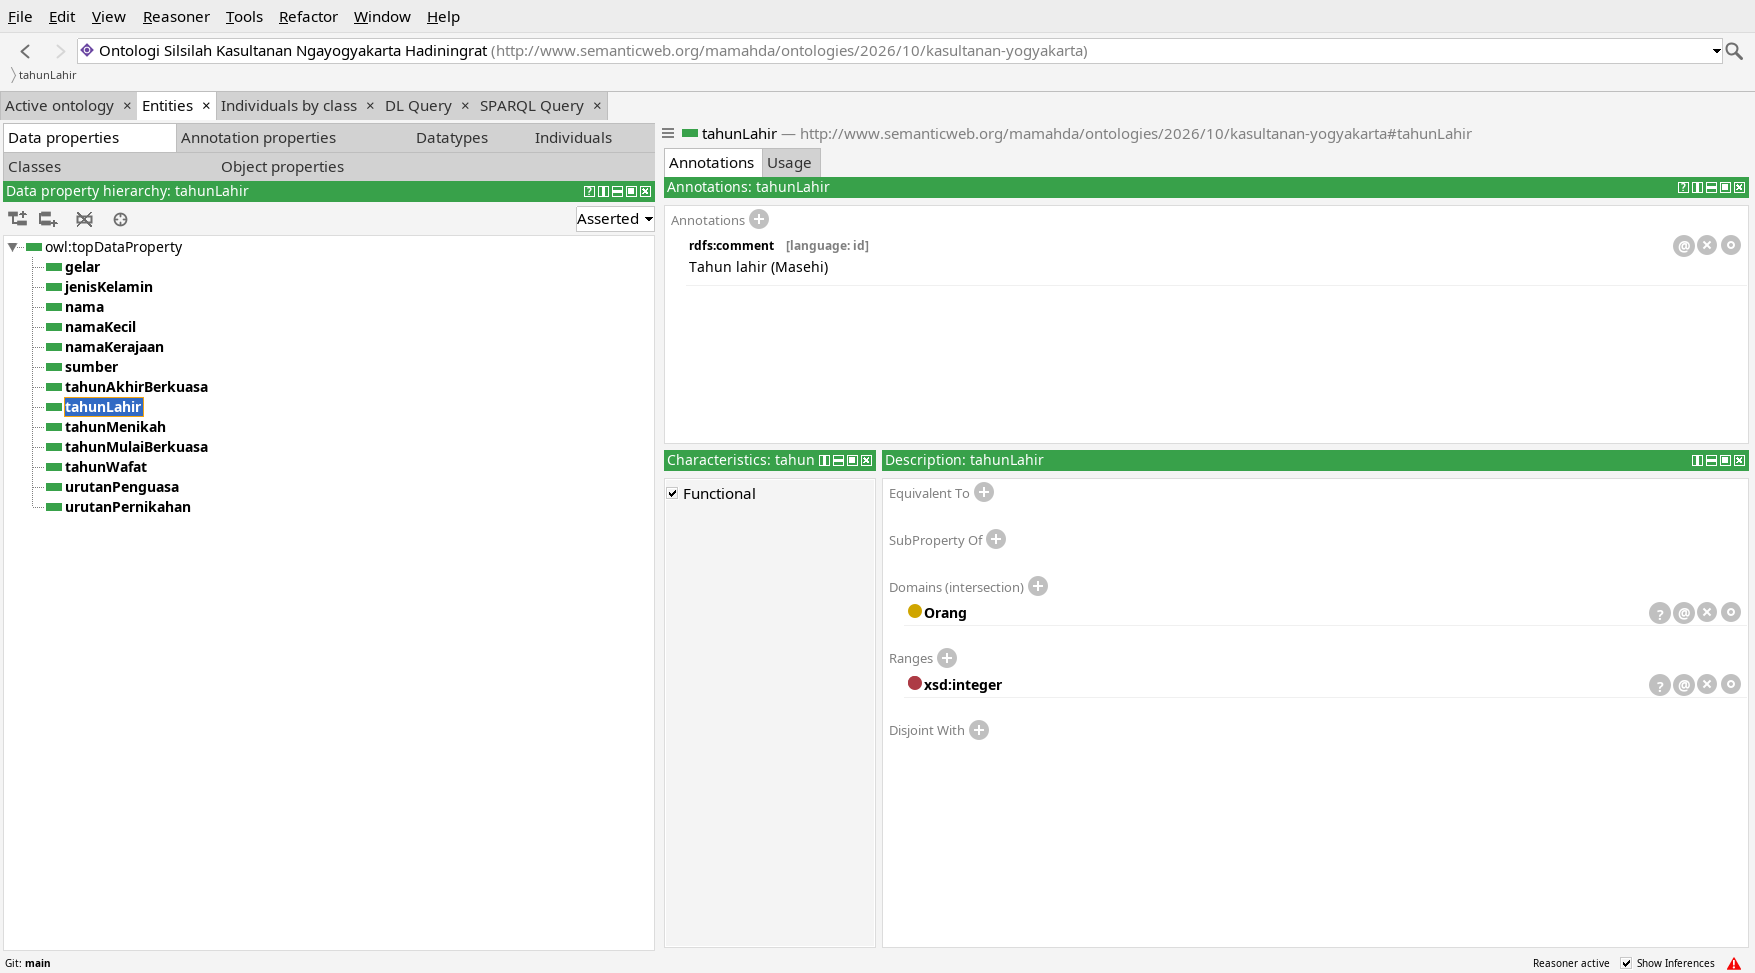
\includegraphics[width=\textwidth]{gambar/data_property.png}
\caption{Daftar \textit{data property} di Prot\'eg\'e.}
\label{fig:ss-data}
\end{figure}

\subsection{Hasil Inferensi Reasoner}

Setelah HermiT dijalankan, ontologi dinyatakan konsisten. Relasi hasil inferensi ditampilkan Prot\'eg\'e dengan latar
kuning. Gambar~\ref{fig:ss-hbx} menunjukkan inferensi dari \textit{inverse property}: HB Ka 10 \texttt{ayahDari} kelima
putrinya dan \texttt{menggantikan} HB IX, padahal yang ditulis di ontologi hanya \texttt{punyaAyah} dan \texttt{digantikanOleh}.
Gambar~\ref{fig:ss-manteyyo} menunjukkan inferensi properti transitif: RM Manteyyo hanya memiliki fakta \texttt{punyaAyah}
dan \texttt{punyaIbu}, tetapi \textit{reasoner} menyimpulkan seluruh leluhurnya sampai HB I dan Sunan Amangkurat IV.

\begin{figure}[H]
\centering
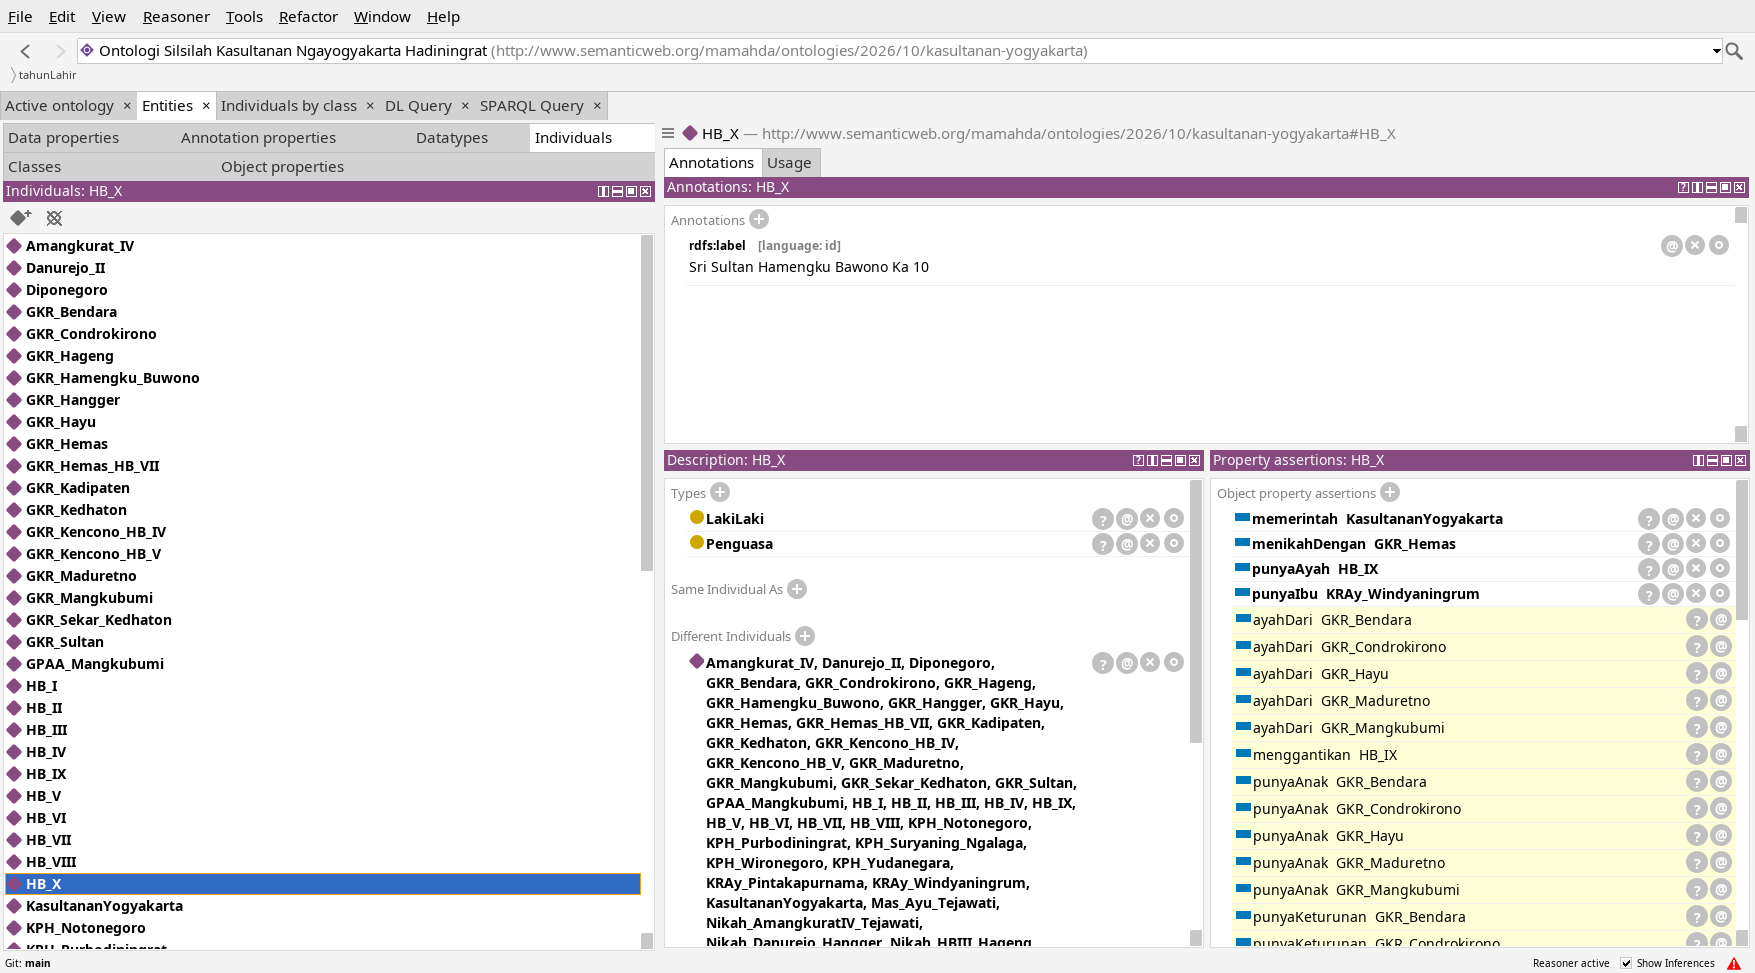
\includegraphics[width=\textwidth]{gambar/individu_HBX.png}
\caption{Individu \texttt{HB\_X}: fakta yang ditulis (huruf tebal) dan hasil inferensi (latar kuning).}
\label{fig:ss-hbx}
\end{figure}

\begin{figure}[H]
\centering
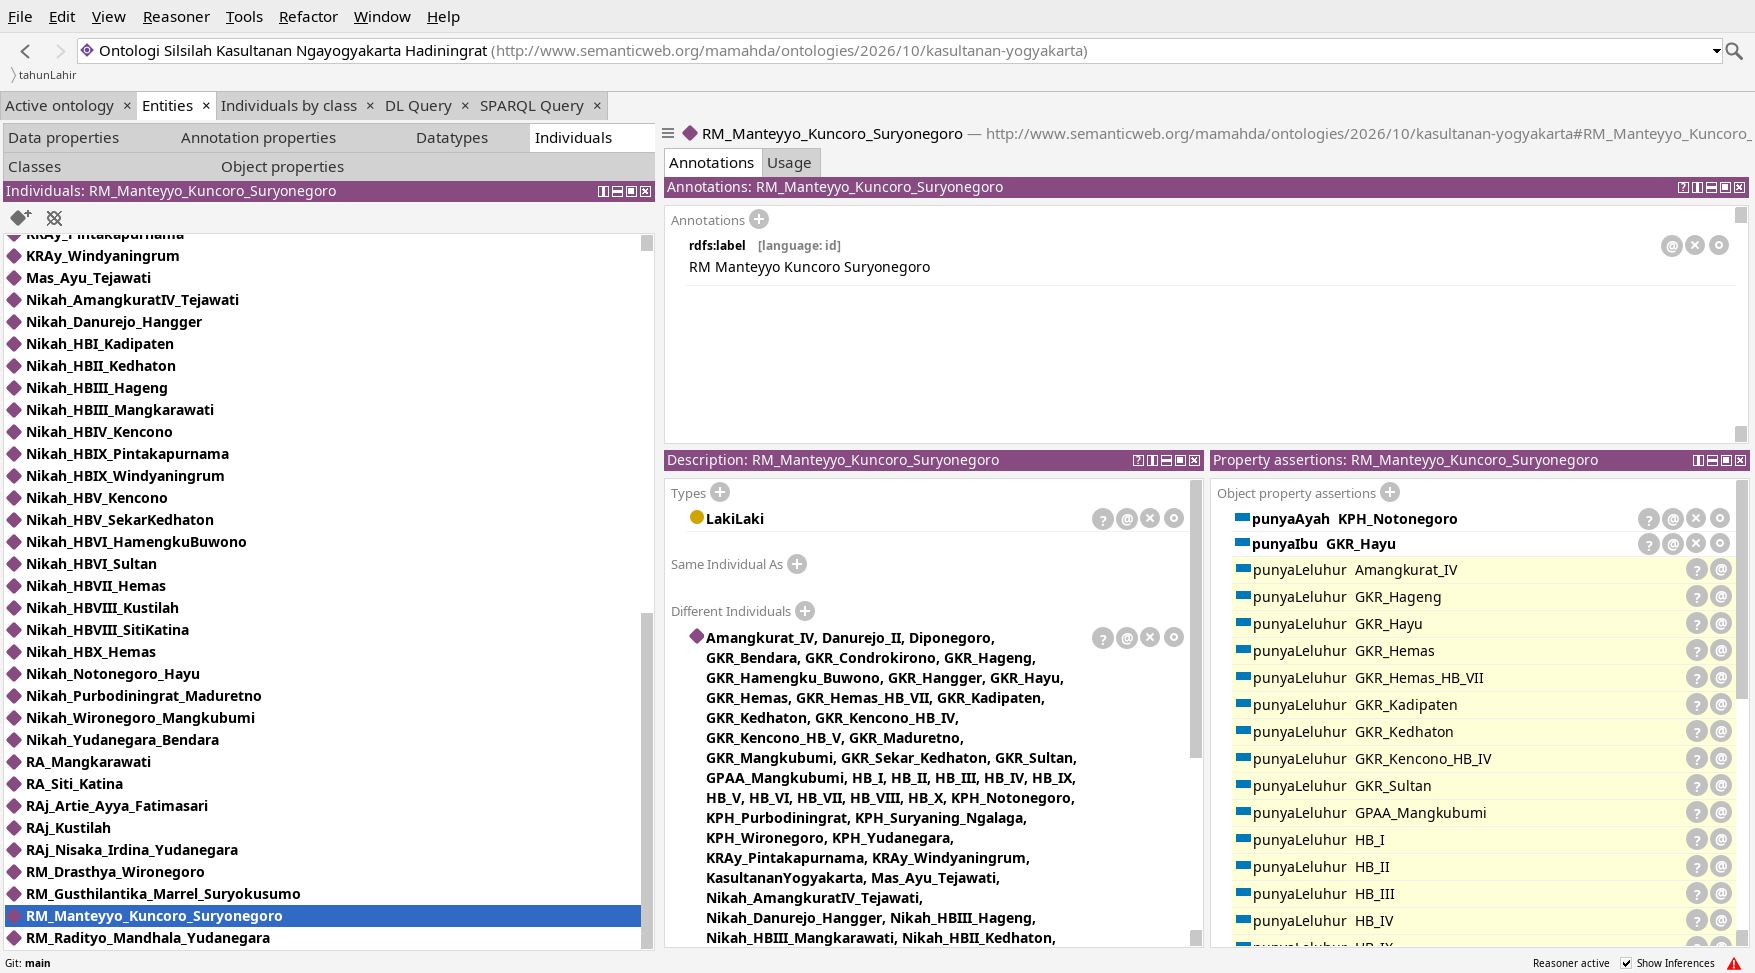
\includegraphics[width=\textwidth]{gambar/individu_Manteyyo.png}
\caption{Individu \texttt{RM\_Manteyyo\_Kuncoro\_Suryonegoro}: \texttt{punyaLeluhur} hasil inferensi properti transitif.}
\label{fig:ss-manteyyo}
\end{figure}

% ================================================================ 5. HASIL SPARQL
\section{Hasil SPARQL}

Query dijalankan di Prot\'eg\'e 5.6.9 dengan \textit{plugin} Snap SPARQL Query 6.0.0. Tab SPARQL Query bawaan tidak
dipakai karena tidak berfungsi di Prot\'eg\'e 5.6.x (galat \texttt{NoClassDefFoundError} pada \textit{plugin} rdf-library).
Snap SPARQL tidak mendukung \textit{property path}, sehingga relasi cucu pada query (c) ditulis dengan gabungan pola
\texttt{UNION}. Semua query hanya memakai fakta yang ditulis langsung di ontologi, sehingga hasilnya sama dengan atau
tanpa \textit{reasoner}.

\subsection{Query (a): Penguasa yang Ayahnya Pernah Menjadi Penguasa}

\textbf{Pertanyaan:} Tampilkan nama penguasa, jenis kelamin penguasa, dan nama ayah, dengan syarat sang ayah pernah
menjadi penguasa sebelumnya.

\begin{lstlisting}
PREFIX rdf: <http://www.w3.org/1999/02/22-rdf-syntax-ns#>
PREFIX : <http://www.semanticweb.org/mamahda/ontologies/2026/10/kasultanan-yogyakarta#>

SELECT ?namaPenguasa ?jenisKelamin ?namaAyah
WHERE {
    ?penguasa rdf:type :Penguasa ;
              :nama ?namaPenguasa ;
              :jenisKelamin ?jenisKelamin ;
              :tahunMulaiBerkuasa ?mulaiAnak ;
              :punyaAyah ?ayah .
    ?ayah rdf:type :Penguasa ;
          :nama ?namaAyah ;
          :tahunMulaiBerkuasa ?mulaiAyah .
    FILTER (?mulaiAyah < ?mulaiAnak)
}
ORDER BY ?mulaiAnak
\end{lstlisting}

\begin{figure}[H]
\centering
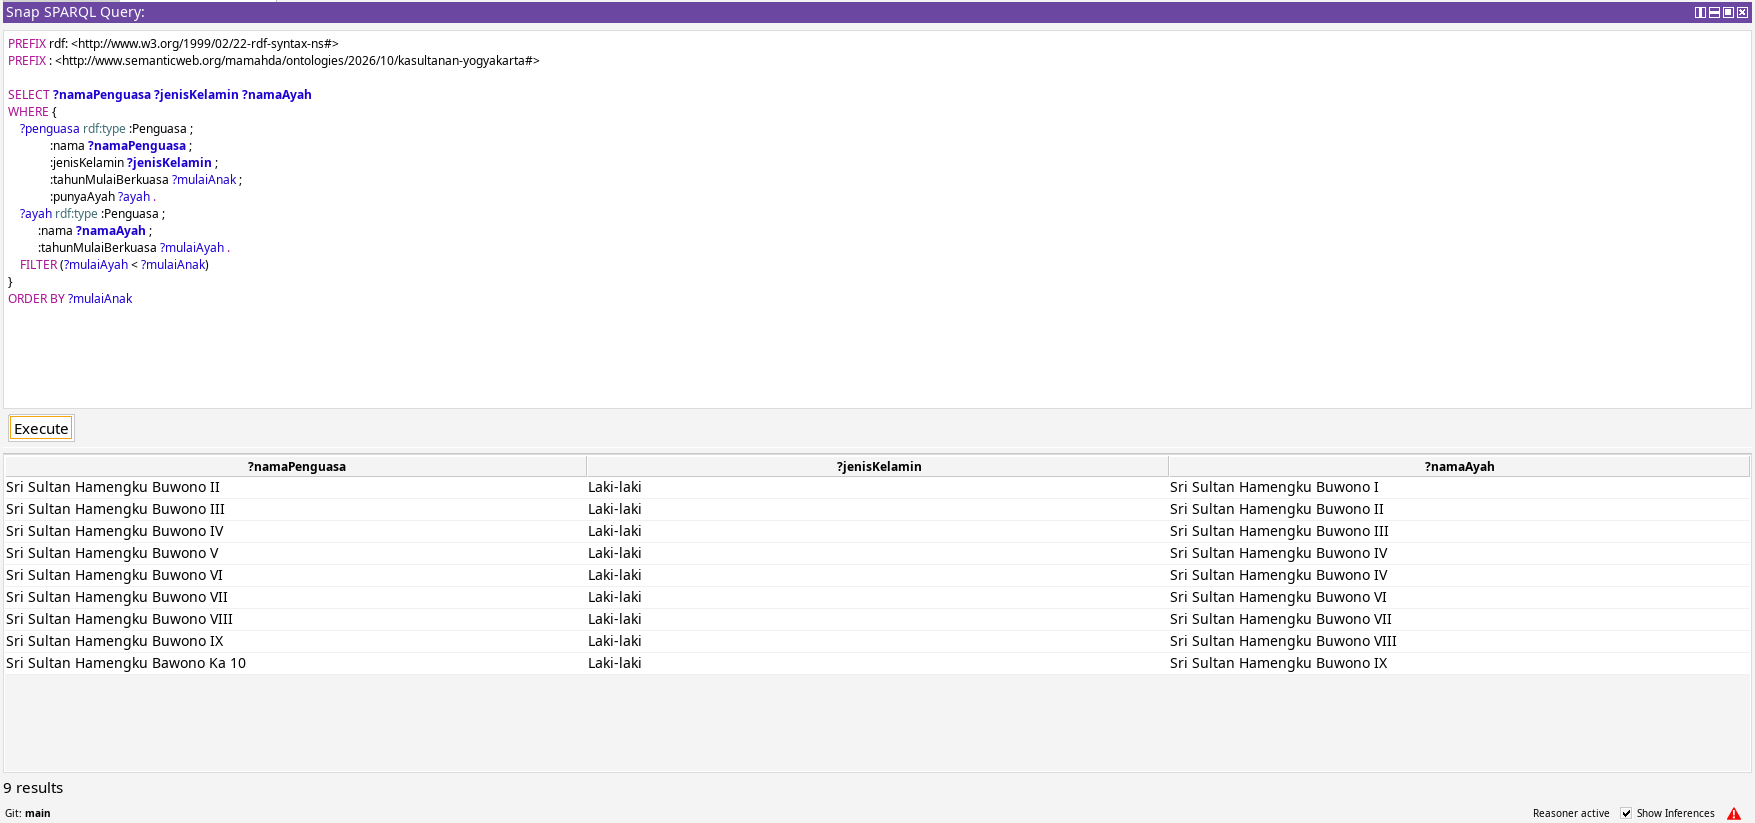
\includegraphics[width=\textwidth]{gambar/query_a.png}
\caption{Hasil query (a): 9 baris.}
\label{fig:qa}
\end{figure}

Query menghasilkan 9 baris, yaitu HB II sampai HB Ka 10. Syarat ``sebelumnya'' dipastikan dengan membandingkan
\texttt{tahunMulaiBerkuasa} ayah dan anak. HB I tidak muncul karena ayahnya, Sunan Amangkurat IV, bukan penguasa
Kasultanan Yogyakarta. HB V dan HB VI sama-sama muncul dengan ayah HB IV karena keduanya bersaudara.

\subsection{Query (b): Anak dari Pernikahan Pertama}

\textbf{Pertanyaan:} Tampilkan nama anak, nama ayah, nama ibu, dan tahun lahir masing-masing orang tua pada pernikahan
pertama. Jika tahun lahir tidak tercatat, data anak tetap ditampilkan dengan kolom tahun lahir kosong.

\begin{lstlisting}
PREFIX rdf: <http://www.w3.org/1999/02/22-rdf-syntax-ns#>
PREFIX : <http://www.semanticweb.org/mamahda/ontologies/2026/10/kasultanan-yogyakarta#>

SELECT ?namaAnak ?namaAyah ?tahunLahirAyah ?namaIbu ?tahunLahirIbu
WHERE {
    ?nikah rdf:type :Pernikahan ;
           :suami ?ayah ;
           :istri ?ibu ;
           :urutanPernikahan 1 .
    ?anak :punyaAyah ?ayah ;
          :punyaIbu ?ibu ;
          :nama ?namaAnak .
    ?ayah :nama ?namaAyah .
    ?ibu  :nama ?namaIbu .
    OPTIONAL { ?ayah :tahunLahir ?tahunLahirAyah . }
    OPTIONAL { ?ibu  :tahunLahir ?tahunLahirIbu . }
}
ORDER BY ?namaAyah ?namaAnak
\end{lstlisting}

\begin{figure}[H]
\centering
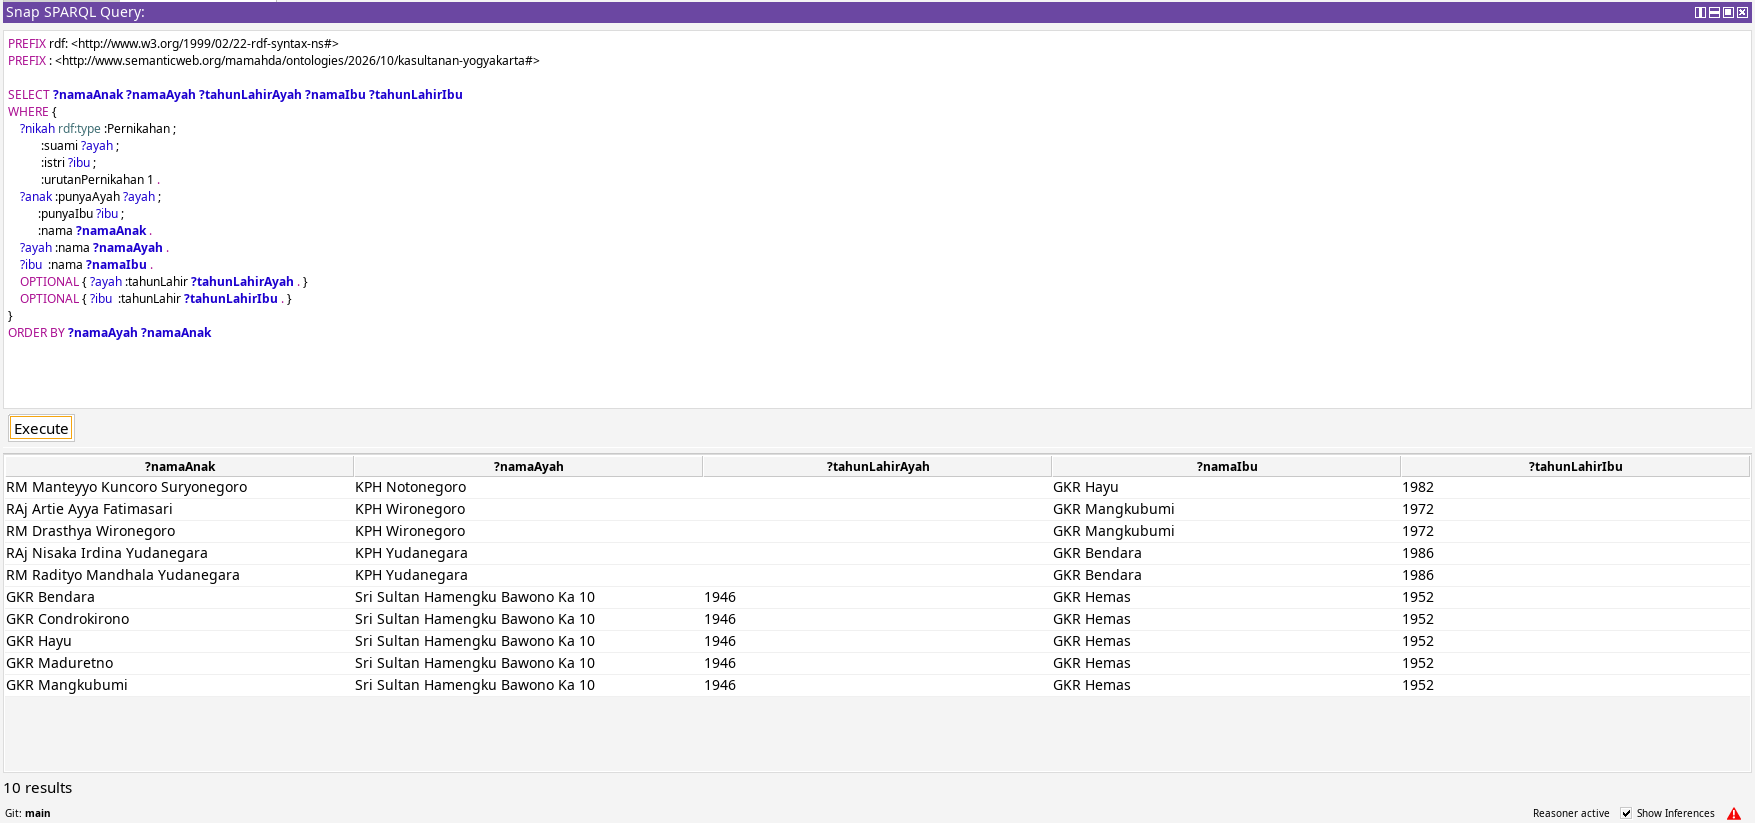
\includegraphics[width=\textwidth]{gambar/query_b.png}
\caption{Hasil query (b): 10 baris.}
\label{fig:qb}
\end{figure}

Query menghasilkan 10 baris: lima putri dari pernikahan HB Ka 10 dengan GKR Hemas, serta cucu-cucu dari pernikahan putri
HB Ka 10. Tahun lahir para menantu tidak tercatat di sumber. Karena tahun lahir diambil dengan \texttt{OPTIONAL}, baris
anaknya tetap muncul dengan kolom tahun lahir ayah kosong, sesuai syarat soal.

Anak HB V, HB VI, HB VIII, dan HB IX tidak muncul. Pernikahan pertama HB V dengan GKR Kencono tidak berputra
\cite{kj-hb5}, sedangkan anak dari pernikahan pertama HB VI, HB VIII, dan HB IX tidak tercatat di sumber. Anak-anak
yang tercatat (KPH Suryaning Ngalaga, HB VII, HB IX, HB Ka 10) lahir dari pernikahan berikutnya. Pernikahan yang
urutannya tidak disebut di sumber, misalnya HB II dengan GKR Kedhaton, tidak diberi nilai \texttt{urutanPernikahan},
sehingga anaknya juga tidak ikut ditampilkan.

\subsection{Query (c): Cucu Penguasa Generasi Pertama}

\textbf{Pertanyaan:} Tampilkan nama cucu dan tahun lahir dari penguasa generasi pertama, diurutkan berdasarkan tahun lahir.

\begin{lstlisting}
PREFIX rdf: <http://www.w3.org/1999/02/22-rdf-syntax-ns#>
PREFIX : <http://www.semanticweb.org/mamahda/ontologies/2026/10/kasultanan-yogyakarta#>

SELECT DISTINCT ?namaCucu ?tahunLahir
WHERE {
    ?penguasa rdf:type :Penguasa ;
              :urutanPenguasa 1 .
    { ?anak :punyaAyah ?penguasa . } UNION { ?anak :punyaIbu ?penguasa . }
    { ?cucu :punyaAyah ?anak . }     UNION { ?cucu :punyaIbu ?anak . }
    ?cucu :nama ?namaCucu .
    OPTIONAL { ?cucu :tahunLahir ?tahunLahir . }
}
ORDER BY ?tahunLahir
\end{lstlisting}

\begin{figure}[H]
\centering
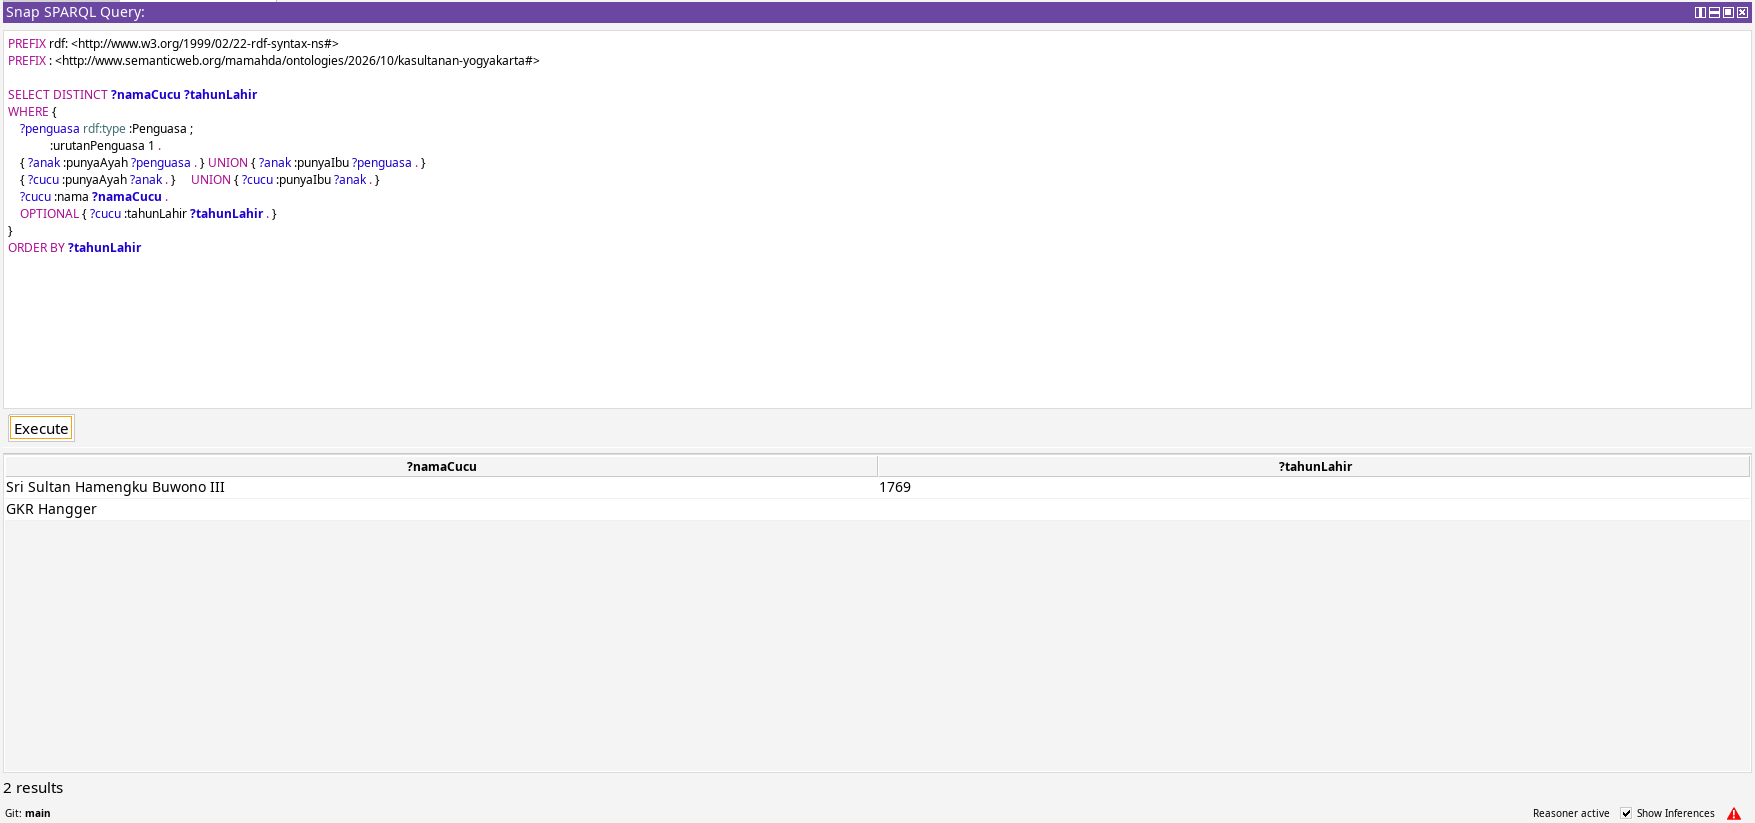
\includegraphics[width=\textwidth]{gambar/query_c.png}
\caption{Hasil query (c): 2 baris.}
\label{fig:qc}
\end{figure}

Penguasa generasi pertama adalah HB I (\texttt{urutanPenguasa} = 1). Cucu yang tercatat adalah HB III (lahir 1769) dan
GKR Hangger, yang tahun lahirnya tidak tercatat. Keduanya anak HB II dan GKR Kedhaton.

\subsection{Query (d): Pasangan Sepupu yang Ayahnya Bersaudara}

\textbf{Pertanyaan:} Tampilkan nama pasangan (laki-laki dan perempuan) yang merupakan sepupu yang tidak boleh menikah,
yaitu sepupu yang ayahnya bersaudara.

\begin{lstlisting}
PREFIX rdf: <http://www.w3.org/1999/02/22-rdf-syntax-ns#>
PREFIX : <http://www.semanticweb.org/mamahda/ontologies/2026/10/kasultanan-yogyakarta#>

SELECT DISTINCT ?namaLakiLaki ?namaPerempuan ?ayahLakiLaki ?ayahPerempuan ?kakekBersama
WHERE {
    ?laki rdf:type :LakiLaki ;
          :menikahDengan ?perempuan ;
          :punyaAyah ?aL ;
          :nama ?namaLakiLaki .
    ?perempuan rdf:type :Perempuan ;
               :punyaAyah ?aP ;
               :nama ?namaPerempuan .
    ?aL :punyaAyah ?kakek ; :nama ?ayahLakiLaki .
    ?aP :punyaAyah ?kakek ; :nama ?ayahPerempuan .
    ?kakek :nama ?kakekBersama .
    FILTER (?aL != ?aP)
}
\end{lstlisting}

\begin{figure}[H]
\centering
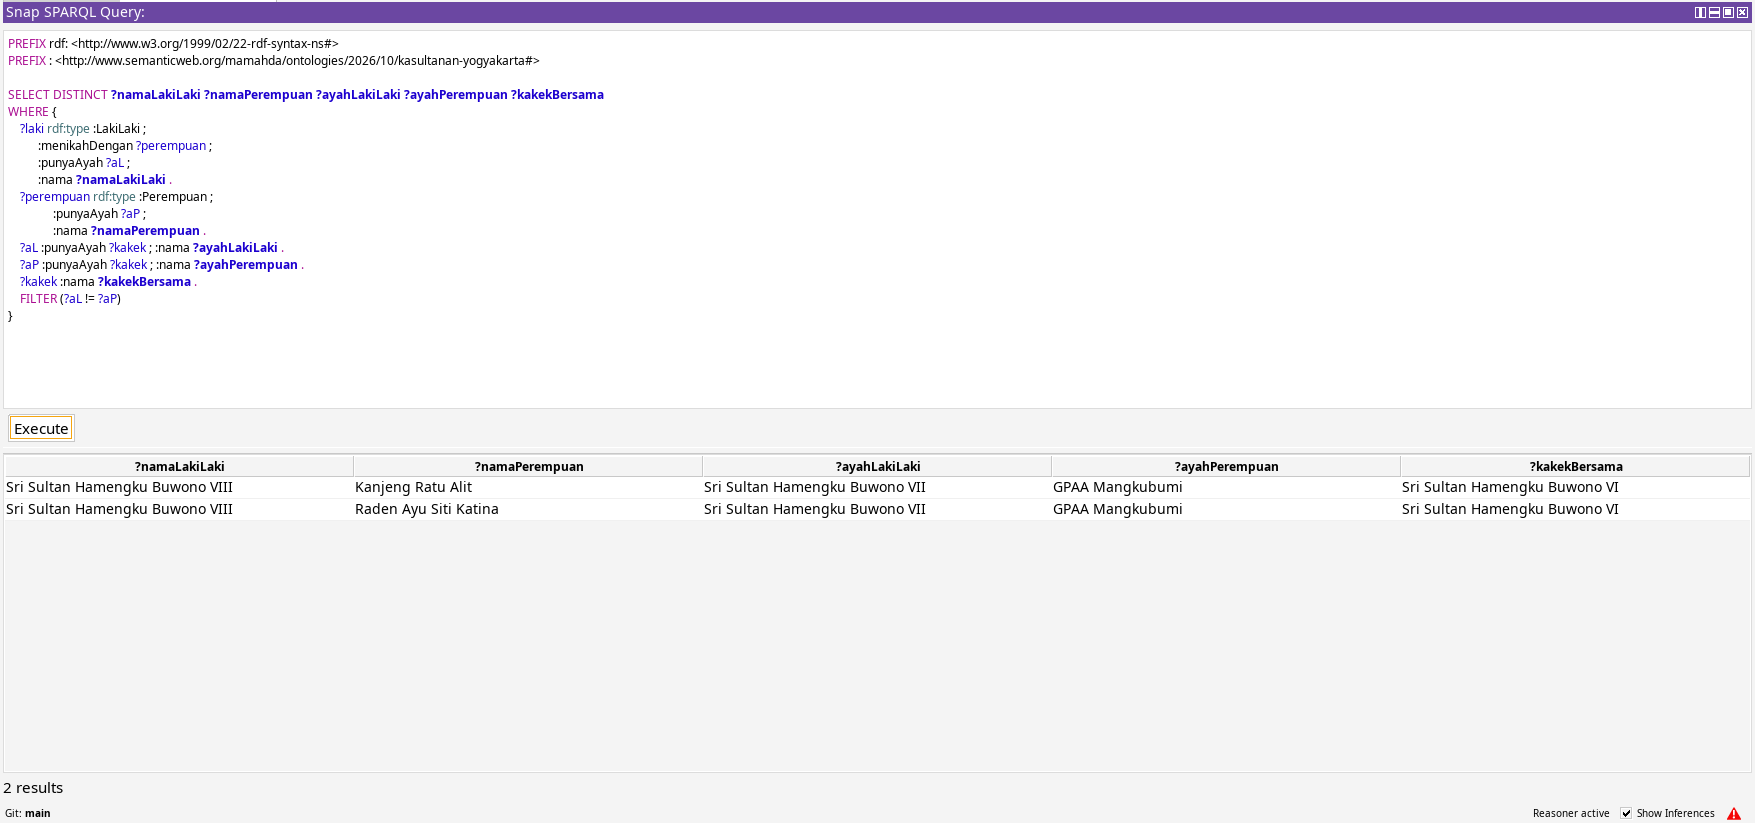
\includegraphics[width=\textwidth]{gambar/query_d.png}
\caption{Hasil query (d): 2 baris.}
\label{fig:qd}
\end{figure}

Hasilnya dua pasangan: Sri Sultan Hamengku Buwono VIII dengan Kanjeng Ratu Alit, dan Sri Sultan Hamengku Buwono VIII
dengan Raden Ayu Siti Katina. Ayah HB VIII (HB VII) dan ayah kedua istri tersebut (GPAA Mangkubumi) sama-sama putra HB VI
\cite{ra-y6,wiki-hb8}. \texttt{FILTER (?aL != ?aP)} memastikan kedua ayah adalah orang yang berbeda, sehingga pasangan
yang dihasilkan adalah sepupu, bukan saudara kandung.

\subsection{Query (e): Putra-Putri Sultan yang Tidak Naik Takhta}

\textbf{Pertanyaan kelompok:} Tampilkan putra-putri Sultan, yaitu anak dari seorang Sultan \emph{atau} anak dari seorang
Permaisuri, yang tidak pernah naik takhta. Sertakan nama orang tua yang menghubungkannya dan tahun lahir jika tercatat.

\begin{lstlisting}
PREFIX rdf: <http://www.w3.org/1999/02/22-rdf-syntax-ns#>
PREFIX : <http://www.semanticweb.org/mamahda/ontologies/2026/10/kasultanan-yogyakarta#>

SELECT DISTINCT ?nama ?jenisKelamin ?namaOrangTua ?tahunLahir
WHERE {
    {
        ?anak :punyaAyah ?ortu .
        ?ortu rdf:type :Penguasa .
    }
    UNION
    {
        ?anak :punyaIbu ?ortu .
        ?ortu rdf:type :Permaisuri .
    }
    ?anak :nama ?nama ;
          :jenisKelamin ?jenisKelamin .
    ?ortu :nama ?namaOrangTua .
    OPTIONAL { ?anak :tahunLahir ?tahunLahir . }
    MINUS { ?anak rdf:type :Penguasa . }
}
ORDER BY ?nama ?namaOrangTua
\end{lstlisting}

\begin{itemize}
  \item \texttt{UNION} menggabungkan dua jalur: anak lewat ayah yang bertipe \texttt{Penguasa}, atau anak lewat ibu yang bertipe \texttt{Permaisuri}.
  \item \texttt{OPTIONAL} dipakai untuk tahun lahir, yang tidak selalu tercatat.
  \item \texttt{MINUS} membuang anak yang bertipe \texttt{Penguasa}, yaitu yang pernah naik takhta.
\end{itemize}

\begin{figure}[H]
\centering
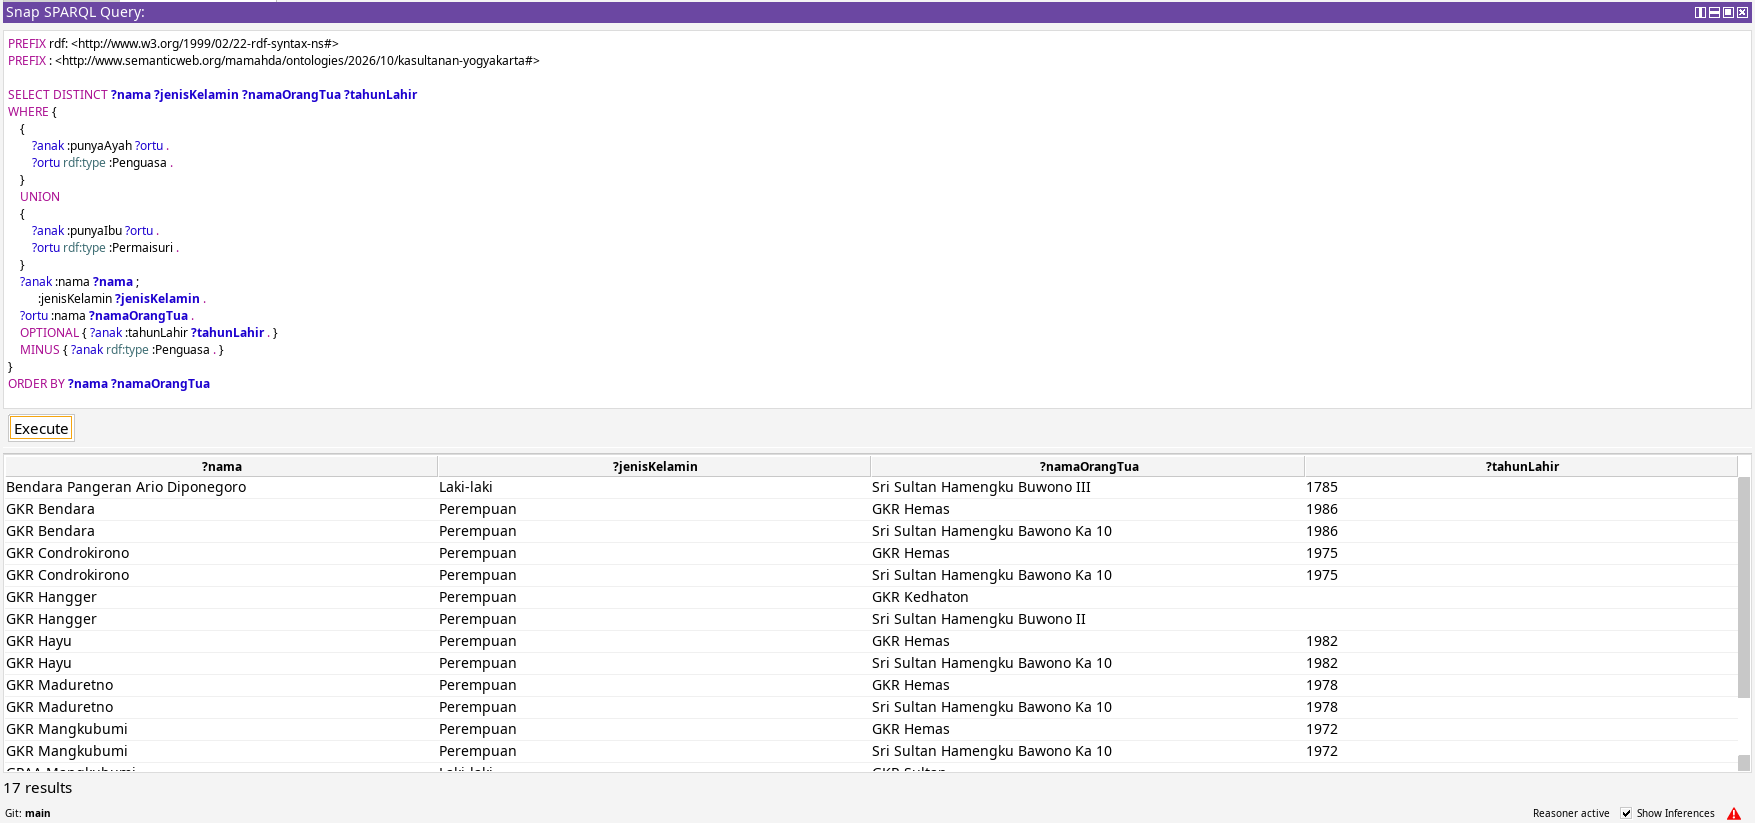
\includegraphics[width=\textwidth]{gambar/query_e.png}
\caption{Query (e) di Snap SPARQL.}
\label{fig:qe}
\end{figure}

\begin{figure}[H]
\centering
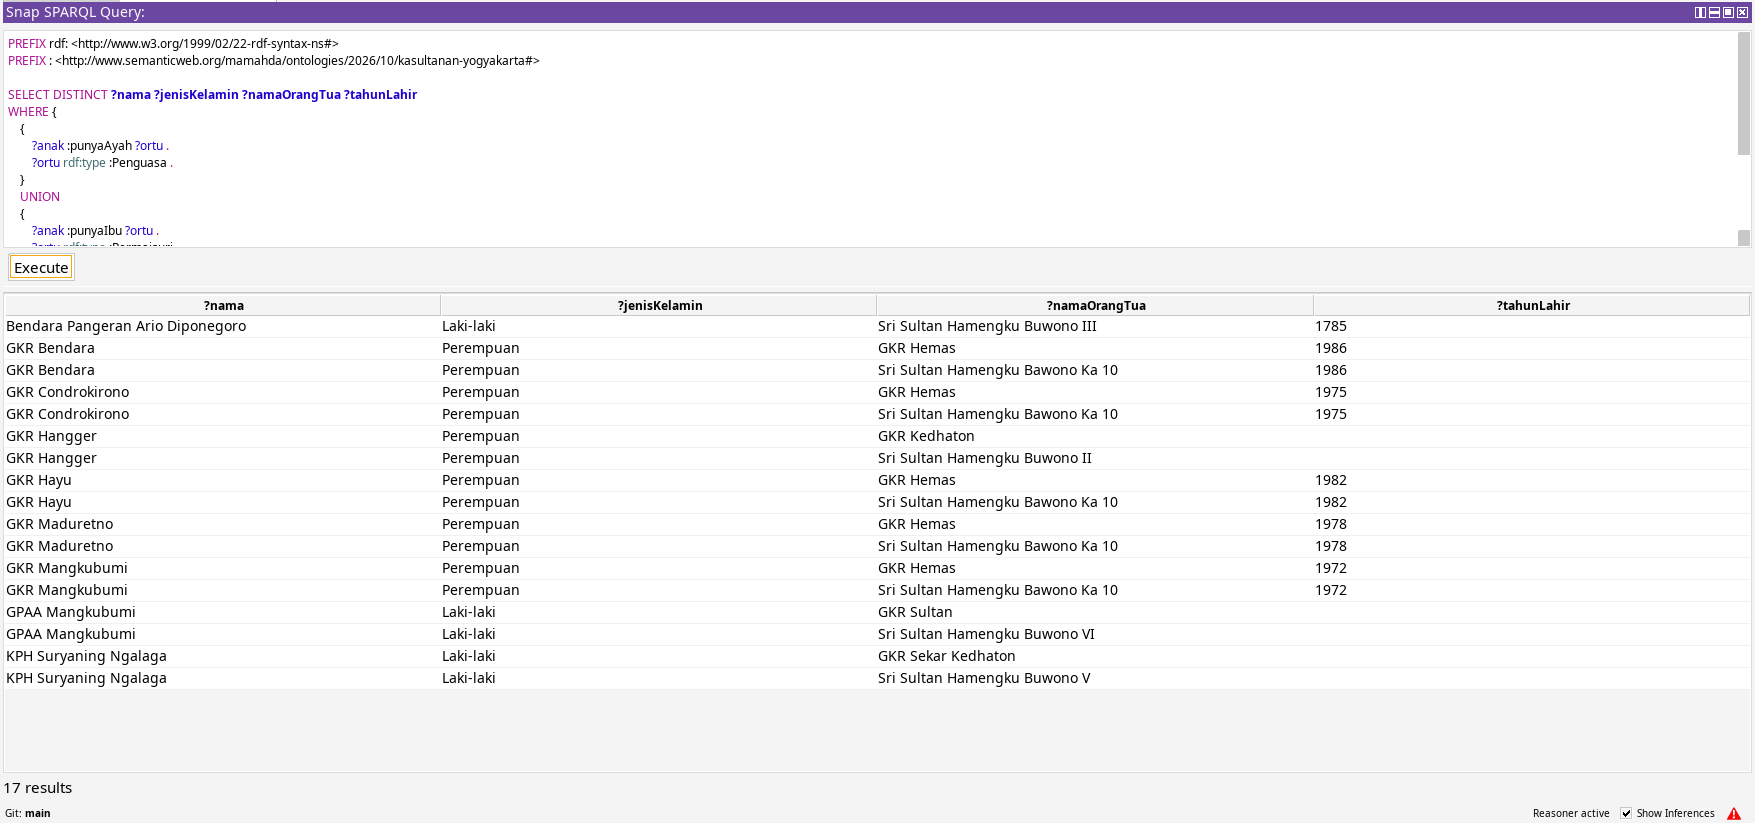
\includegraphics[width=\textwidth]{gambar/query_e_hasil.png}
\caption{Hasil lengkap query (e): 17 baris.}
\label{fig:qe2}
\end{figure}

Query menghasilkan 17 baris. Setiap anak muncul dua kali (sekali lewat ayah, sekali lewat ibu), kecuali Pangeran
Diponegoro. Ibunya, R.A. Mangkarawati, adalah garwa selir, bukan Permaisuri, sehingga Diponegoro hanya ditemukan lewat
jalur ayah.

% ================================================================ 6. DAFTAR PUSTAKA
\begin{thebibliography}{99}
\raggedright
\addcontentsline{toc}{section}{Daftar Pustaka}

\bibitem{kj-hb1} Kraton Jogja, ``Sri Sultan Hamengku Buwono I,'' \emph{kratonjogja.id}. [Online]. Available: \url{https://www.kratonjogja.id}. [Accessed: Oct. 19, 2026].

\bibitem{kj-hb2} Kraton Jogja, ``Sri Sultan Hamengku Buwono II,'' \emph{kratonjogja.id}. [Online]. Available: \url{https://www.kratonjogja.id}. [Accessed: Oct. 19, 2026].

\bibitem{kj-hb3} Kraton Jogja, ``Sri Sultan Hamengku Buwono III,'' \emph{kratonjogja.id}. [Online]. Available: \url{https://www.kratonjogja.id}. [Accessed: Oct. 19, 2026].

\bibitem{kj-hb4} Kraton Jogja, ``Sri Sultan Hamengku Buwono IV,'' \emph{kratonjogja.id}. [Online]. Available: \url{https://www.kratonjogja.id}. [Accessed: Oct. 19, 2026].

\bibitem{kj-hb5} Kraton Jogja, ``Sri Sultan Hamengku Buwono V,'' \emph{kratonjogja.id}. [Online]. Available: \url{https://www.kratonjogja.id}. [Accessed: Oct. 19, 2026].

\bibitem{kj-hb6} Kraton Jogja, ``Sri Sultan Hamengku Buwono VI,'' \emph{kratonjogja.id}. [Online]. Available: \url{https://www.kratonjogja.id}. [Accessed: Oct. 19, 2026].

\bibitem{kj-hb7} Kraton Jogja, ``Sri Sultan Hamengku Buwono VII,'' \emph{kratonjogja.id}. [Online]. Available: \url{https://www.kratonjogja.id}. [Accessed: Oct. 19, 2026].

\bibitem{kj-hb8} Kraton Jogja, ``Sri Sultan Hamengku Buwono VIII,'' \emph{kratonjogja.id}. [Online]. Available: \url{https://www.kratonjogja.id}. [Accessed: Oct. 19, 2026].

\bibitem{kj-hb9} Kraton Jogja, ``Sri Sultan Hamengku Buwono IX,'' \emph{kratonjogja.id}. [Online]. Available: \url{https://www.kratonjogja.id}. [Accessed: Oct. 19, 2026].

\bibitem{kj-bertakhta} Kraton Jogja, ``Yang Bertakhta,'' \emph{kratonjogja.id}. [Online]. Available: \url{https://www.kratonjogja.id}. [Accessed: Oct. 19, 2026].

\bibitem{kj-hayu} Kraton Jogja, ``Gusti Kanjeng Ratu Hayu, Menjaga Tradisi dengan Teknologi,'' \emph{kratonjogja.id}. [Online]. Available: \url{https://www.kratonjogja.id}. [Accessed: Oct. 19, 2026].

\bibitem{kj-maduretno} Kraton Jogja, ``GKR Maduretno, Putri Tengah yang Dekat dengan Sang Ayah,'' \emph{kratonjogja.id}. [Online]. Available: \url{https://www.kratonjogja.id}. [Accessed: Oct. 19, 2026].

\bibitem{kj-hemas} Kraton Jogja, ``GKR Hemas, Kekuatan Perempuan untuk Kebaikan,'' \emph{kratonjogja.id}. [Online]. Available: \url{https://www.kratonjogja.id}. [Accessed: Oct. 19, 2026].

\bibitem{kj-pepatih} Kraton Jogja, ``Pepatih Dalem Kesultanan Yogyakarta,'' \emph{kratonjogja.id}. [Online]. Available: \url{https://www.kratonjogja.id}. [Accessed: Oct. 19, 2026].

\bibitem{kj-nisaka} Kraton Jogja, ``Memasuki Masa Remaja, RAj Nisaka Irdina Yudanegara Jalani Upacara Tarapan,'' \emph{kratonjogja.id}, Sep. 30, 2023. [Online]. Available: \url{https://www.kratonjogja.id}. [Accessed: Oct. 19, 2026].

\bibitem{wiki-hb8} ``Hamengkubuwana VIII,'' \emph{Wikipedia bahasa Indonesia}. [Online]. Available: \url{https://id.wikipedia.org}. [Accessed: Oct. 19, 2026].

\bibitem{wiki-hb9} ``Hamengkubuwana IX,'' \emph{Wikipedia bahasa Indonesia}. [Online]. Available: \url{https://id.wikipedia.org}. [Accessed: Oct. 19, 2026].

\bibitem{wiki-hb10} ``Hamengkubuwana X,'' \emph{Wikipedia bahasa Indonesia}. [Online]. Available: \url{https://id.wikipedia.org}. [Accessed: Oct. 19, 2026].

\bibitem{wiki-dipo} ``Diponegoro,'' \emph{Wikipedia bahasa Indonesia}. [Online]. Available: \url{https://id.wikipedia.org}. [Accessed: Oct. 19, 2026].

\bibitem{wiki-hemas} ``Gusti Kanjeng Ratu Hemas,'' \emph{Wikipedia bahasa Indonesia}. [Online]. Available: \url{https://id.wikipedia.org}. [Accessed: Oct. 19, 2026].

\bibitem{ra-y6} C. Buyers, ``Yogyakarta: Genealogy (part 6),'' \emph{The Royal Ark}. [Online]. Available: \url{https://www.royalark.net}. [Accessed: Oct. 19, 2026].

\bibitem{ra-y7} C. Buyers, ``Yogyakarta: Genealogy (part 7),'' \emph{The Royal Ark}. [Online]. Available: \url{https://www.royalark.net}. [Accessed: Oct. 19, 2026].

\bibitem{ra-y8} C. Buyers, ``Yogyakarta: Genealogy (part 8),'' \emph{The Royal Ark}. [Online]. Available: \url{https://www.royalark.net}. [Accessed: Oct. 19, 2026].

\end{thebibliography}

\end{document}
